\documentclass[11pt, a4paper, oneside]{Thesis} % Paper size, default font size and one-sided paper

\graphicspath{{./Pictures/}} % Specifies the directory where pictures are stored
\usepackage{cite}
\usepackage{graphicx}
\usepackage[square, numbers, comma, sort&compress]{natbib} % Use the natbib reference package - read up on this to edit the reference style; if you want text (e.g. Smith et al., 2012) for the in-text references (instead of numbers), remove 'numbers' 
\usepackage[table]{xcolor}
\hypersetup{urlcolor=blue, colorlinks=true} % Colors hyperlinks in blue - change to black if annoying
\title{\ttitle} % Defines the thesis title - don't touch this

\begin{document}

\frontmatter % Use roman page numbering style (i, ii, iii, iv...) for the pre-content pages

\setstretch{1.3} % Line spacing of 1.3

% Define the page headers using the FancyHdr package and set up for one-sided printing
\fancyhead{} % Clears all page headers and footers
\fancyfoot[RO, LE] {\thepage}
\rhead{} % Sets the right side header to show the page number
\lhead{} % Clears the left side page header
\pagestyle{fancy} % Finally, use the "fancy" page style to implement the FancyHdr headers

\newcommand{\HRule}{\rule{\linewidth}{0.5mm}} % New command to make the lines in the title page

\definecolor{colTabla}{rgb}{0.33,0.55,0.83}
\definecolor{colFila}{rgb}{0.78,0.85,0.95}

\hypersetup{pdftitle={\ttitle}}
\hypersetup{pdfsubject=\subjectname}
\hypersetup{pdfauthor=\authornames}
\hypersetup{pdfkeywords=\keywordnames}

%----------------------------------------------------------------------------------------
%	TITLE PAGE
%----------------------------------------------------------------------------------------

\begin{titlepage}
\begin{center}

\textsc{\huge \tilsor}\\[2.0cm] % University name
\textsc{\huge \udelar}\\[1.5cm] % University name
\textsc{\LARGE \fing}\\[1.5cm] % University name
\textsc{\Large Tesis de grado}\\[0.5cm] % Thesis type

\HRule \\[0.4cm] % Horizontal line
{\huge \bfseries \ttitle}\\[0.4cm] % Thesis title
\HRule \\[1.5cm] % Horizontal line
 
\begin{minipage}{0.4\textwidth}
\begin{flushleft} \large
\emph{Autor:}\\
{\authornames}\\
\bigskip
\emph{Contraparte del cliente:}\\
{\fmolina} 
\end{flushleft}
\end{minipage}
\begin{minipage}{0.4\textwidth}
\begin{flushright} \large
\emph{Supervisor:} \\
{\gustun}\\
\bigskip
\emph{Supervisor alterno:} \\
{\marcelor}
\end{flushright}
\end{minipage}\\[3cm]
 
{\large \today}\\[4cm] % Date
%\includegraphics{Logo} % University/department logo - uncomment to place it
 
\vfill
\end{center}

\end{titlepage}

%----------------------------------------------------------------------------------------
%	LIST OF CONTENTS/FIGURES/TABLES PAGES
%----------------------------------------------------------------------------------------

\pagestyle{fancy} % The page style headers have been "empty" all this time, now use the "fancy" headers as defined before to bring them back

\lhead{\emph{Contents}} % Set the left side page header to "Contents"
\tableofcontents % Write out the Table of Contents

%\lhead{\emph{List of Figures}} % Set the left side page header to "List of Figures"
%\listoffigures % Write out the List of Figures

%\lhead{\emph{List of Tables}} % Set the left side page header to "List of Tables"
%\listoftables % Write out the List of Tables

%----------------------------------------------------------------------------------------
%	THESIS CONTENT - CHAPTERS
%----------------------------------------------------------------------------------------

\mainmatter % Begin numeric (1,2,3...) page numbering

\pagestyle{fancy} % Return the page headers back to the "fancy" style

% Include the chapters of the thesis as separate files from the Chapters folder
% Uncomment the lines as you write the chapters

% Chapter 1

\chapter{Glosario} % Main chapter title

\lfoot{Glosario}} % This is for the header on each page - perhaps a shortened title

%----------------------------------------------------------------------------------------



\emph{Conceptos utilizados en TAXII}
\begin{itemize}
  \item Botnet: Es una colección de computadoras comprometidas (llamadas computadoras zombie), 
instaladas generalmente mediante gusanos, troyanos y backdoors, controladas 
remotamente, usualmente con fines maliciosos, en especial para denegaciones de 
servicio.
  \item CSIRT: Es una organización responsable de recibir reportes de incidentes de seguridad, analizarlos y responder a ellos. [CERT/CC]
  \item CVE: El CVE (Common Vulnerabilities and Exposures) es un diccionario de comunes (por 
ejemplo los identificadores CVE) para publicar información conocida de 
vulnerabilidades de seguridad. El CCE (Common Configuration Enumeration) provee 
identificadores para problemas de configuración de seguridad. Los 
identificadores hacen más fácil compartir información a través de diferentes 
bases de datos y herramientas de seguridad.
 \item Cyber Threat information: Es cualquier información representable en STIX. 
 Esto incluye, pero no esta limitado a, Observables, Indicadores, incidentes, 
 TTPs (Tactics, Techniques y Procedures), exploit targets, campaigns, threat 
 actors y courses of action.
 \item TAXII Data Feed: Es una colección de cyber threat information 
 estructurada expresable en uno o mas documentos STIX que pueden ser 
 intercambiados utilizando TAXII. Cada TAXII Data Feed \emph{debe} tener un 
 nombre que lo identifica de forma única entre el resto de los feeds de un 
 productor dado. Cada elemento de un TAXII data feed debe ser etiquetado con un 
 timestamp y puede tener otras etiquetas a discreción del productor.
 \item IDS: Intrusion Detection System. Sistema que detecta intrusiones no deseadas en una 
red o equipo, que no pueden ser detectadas por un firewall convencional.
 \item Mensae TAXII: Un bloque de información que es pasado de una entidad a la 
 otra. Un mensaje TAXII representa un pedido o una respuesta.
 \item Intercambio de mensajes TAXII: Una secuencia definida de mensajes TAXII 
 intercambiados entre dos entidades.
\item Servicio TAXII: Son funcionalidades albergadas por algunas entidades y que 
es accedido o invocado usando uno o mas TAXII Message Exchange.
\item TAXII Capability: Una actividad de alto nivel soportado por TAXII por 
medio del uso de uno o mas servicios TAXII.
\end{itemize}




 
% Chapter 1

\chapter{Introducción} % Main chapter title

\label{hola} % For referencing the chapter elsewhere, use \ref{Chapter1} 

\lhead{\til}
\rhead{\fu}
\lfoot{Chapter 1. \emph{Introducción}} % This is for the header on each page - perhaps a shortened title

%----------------------------------------------------------------------------------------

\section{Introducción}
Históricamente, se ha visto un aumento en la sofisticación, velocidad, impacto y 
cantidad de los ataques informáticos. Se ha vuelto necesario que las estrategias 
de defensa se adapten a los nuevos actores y ataques. Para responder a esto, las 
organizaciones han tenido que recurrir al intercambio de información referente a 
las amenazas con el fin de tener una visión más amplia de las actividades de los 
adversarios y así ayudar a administrar sus recursos de forma de obtener el mejor 
resultado posible de sus defensas. Hoy en día el compartir información es realizado 
de forma manual lo cual es una tarea que consume una cantidad de tiempo 
considerable o por medio de procesos automatizados con grandes limitaciones los 
cuales se realizan dentro de comunidades especificas. La capacidad de compartir 
información completa de forma automática con un gran número de comunidades no 
existe en la actualidad. Hay múltiples métodos para el intercambio de 
información y estos juegan un rol significante en los tipos, volúmenes y 
naturaleza de la información compartida con la comunidad. Algunos de estos 
medios de intercambio limitan el tipo de contenido que es compartido de forma 
sencilla mientras que otros promueven ciertos tipos de intercambio. De todas 
formas, la mayoría de estos métodos no permiten el consumo de información de 
amenazas de forma automática, esto hace que rutinariamente las 
organizaciones deban tomar dicha información y sintetizarla en sus bases de 
datos locales. Si bien los métodos utilizados en la actualidad han ayudado a 
mejorar las capacidades defensivas de numerosas organizaciones, estas no han 
logrado explotar su máximo potencial. Por ello es que actualmente existen varios 
esfuerzos para generar arquitecturas abiertas, estándar basadas en indicadores e 
información de incidentes. La realidad es que ninguno de estos ha podido 
convertirse en un estándar para el intercambio entre comunidades.
Las aproximaciones tradicionales de seguridad se focalizan en entender y 
registrar vulnerabilidades, debilidades y configuraciones necesarias pero 
insuficientes. Para defenderse las organizaciones tienen estrategias de defensa 
que buscan predominantemente bloquear los ataques y arreglar 
las vulnerabilidades, esta estrategia se basa en alertas. Si bien puede ser 
efectiva contra algunas amenazas no logra detener ataques avanzados o proveer 
información sobre las actividades de un atacante luego de que la red fue 
penetrada. Una estrategia mas adecuada es basarse en \emph{cyber kill-chain}, en 
esta estrategia se busca descomponer las fases de un ataque con la finalidad de 
obtener una mejor comprensión del ataque y el atacante así como mejorar las 
posibilidades de defensa.

\begin{figure}[ht!]
  \centering
    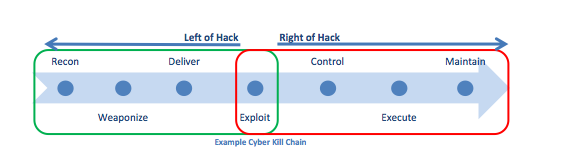
\includegraphics[width=150mm]{./Figures/killChain.png}
\end{figure}

Los primeros pasos de esta estrategia representan una 
oportunidad para detectar y mitigar las amenazas de forma proactiva antes de que 
el adversario realice un acceso no autorizado en los sistemas de la 
organización. En los pasos posteriores es donde se realiza la detección, 
respuesta y aseguramiento de los activos más importantes. Al entender al 
adversario los defensores tienen una mejor oportunidad para descubrir y 
responder al ataque. Un entendimiento de la amenaza permite la realización de 
decisiones mas efectivas, priorizando los recursos para así lograr tener una 
ventaja ante el adversario. El efecto de las defensas en base a inteligencia es 
una mejor postura respecto a las respuestas dado que los atacantes 
ajustan sus operaciones basandose en el éxito o falla de sus intentos. En un 
modelo como el presentado los intentos que realiza un adversario pueden ser 
reconocidos, logrando que los defensores tengan la posibilidad de ajustar sus 
tácticas para una mejor respuesta que genere que el adversario le sea mas 
difícil alcanzar sus objetivos. Compartir información sobre amenazas con socios 
y comunidades de confianza le permite a las organizaciones tener un conjunto de 
información relevante para tener una identificación precisa de una amenaza.
Por el medio de este intercambio, cada ente puede alcanzar un nivel mas alto de 
entendimiento del panorama de las amenazas, no solamente de forma abstracta sino 
que también de evidencias especificas que indiquen la presencia del atacante.
Actualmente se busca que las defensas anticipen y mitiguen 
las amenazas antes de que sean más difíciles de encontrar y erradicar utilizando 
los métodos tradicionales de detección y respuesta. Para poder realizar esto es 
necesario que se realice una actividad de cyber inteligencia recolectando 
información referente a ataques. Con esta información los analistas pueden 
agrupar patrones de actividades similares, atribuir actividades a ciertos 
actores, identificar e implementar estrategias de mitigación de forma rápida y 
anticiparse al lanzamiento de ataques similares en el futuro. Para aprovechar de 
forma más adecuada los beneficios de la cyber inteligencia, las organizaciones 
deben compartir la información recolectada (incluyendo sus estrategias de defensa) 
con socios de su confianza. De esta forma se obtiene una imagen más completa de 
las actividades del adversario y de las acciones defensivas que se deben 
realizar. Por medio del análisis del comportamiento de los adversarios en 
distintos objetivos y en un periodo de tiempo adecuado, los defensores son 
capaces de identificar un conjunto importante de indicadores, tácticas, técnicas 
y procedimientos (TTPs). De esta forma se obtiene información de los objetivos y 
las estrategias lo cual permite al defensor predecir el comportamiento del 
ataque y generar defensas dinámicas. Dada la forma y complejidad con la que 
evoluciona el panorama de las amenazas, la velocidad con la cual ocurren los 
eventos, y la basta cantidad de datos que se deberian intercambiar, es necesario 
establecer una forma automática para ayudar a los analistas y tomadores de 
decisión a tomar acciones defensivas para que esta aproximación sea efectiva. La 
automatización requiere de información de calidad, dado que las arquitecturas 
son heterogéneas con distintos productos y sistemas, es necesario la 
estandarización con representaciones estructuradas de información y un mejor 
aprovechamiento de la información sin saber de antemano quien va a proveer que 
información. Dicha información debe ser legible por un humano y pareseable por 
una máquina. Estos requerimientos tienen varias justificaciones, primer que 
nada, un analista podría realizar un análisis que es inapropiado para ser 
automatizado o que sea focalizados en tomas de decisiones por parte de personas. 
También podría ser de interés que un analista tenga conocimiento de la situación 
actual. Además podría ser un buen medio para evaluar la fidelidad de las fuentes 
y los métodos utilizados para producir la información. Dados todos los factores 
presentados anteriormente, es necesaria la existencia de representaciones 
estructuradas de la información y que esta sea expresiva, flexible, extensible, 
automatizable y legible. Además se deben contar con medios para permitir el 
intercambio seguro y confiable de información entre distintas organizaciones.




\chapter{RTIR} % Main chapter title

\label{Chapter1} % For referencing the chapter elsewhere, use \ref{Chapter1} 

\lhead{\til}
\rhead{\fu}


%----------------------------------------------------------------------------------------

\section{Que es RTIR}
RTIR es un sistema de manejo de incidentes diseñado para ser utilizado por los 
equipos de seguridad de sistemas. A sido creado en conjunto con equipos de CERT 
y CSIRT para manejar el creciente número de incidentes reportados.
Presenta la ventaja de ser opensource, contener una API completa y una comunidad 
de usuarios grande y experta. Además es simple de integrar con otras 
herramientas existentes. Está implementado por medio de módulos PERL y las 
herramientas que provee RT. Se puede pensar en RTIR como una extensión de RT 
para ser utilizada por CERT's y CSIRT's.

Existen algunas alternativas a RTIR como lo son AIRT (Application for Incident Response Teams) 
cuya última versión data de Julio de 2009. AIRT es una aplicación web 
desarrollada para los equipos de respuesta a incidentes. Busca proveer facilidad 
ante los reportes de incidentes de seguridad así como un seguimiento simple de 
estos. Este sistema no cuenta con una comunidad comparable a la de RTIR así como 
con documentación tan extensa como la de RTIR.

Otra de las opciones existentes es OTRS (Open Technology Real Services), así 
como los anteriores también es open soruce. Presenta las ventajas de tener una 
comunidad más numerosa que AIRT y que el código esta siendo desarrollado continuamente. 
Así como RTIR esta desarrollado por medio de Perl y permite conectarse a varias 
bases de datos. Presenta documentación extensa para implementadores.
% Chapter 2

\chapter{TAXII} % Main chapter title

\label{Chapter2} % For referencing the chapter elsewhere, use \ref{Chapter1} 

\lhead{\til}
\rhead{\fu}
\lfoot{Chapter 2. \emph{TAXII}} % This is for the header on each page - perhaps a shortened title

%----------------------------------------------------------------------------------------

\section{Introducción}

A lo largo de la historia de la computación se ha visto un aumento en la 
sofisticación, velocidad e impacto de los ataques informáticos. Se ha vuelto 
necesario que las estrategias de defensa se adapten a los nuevos actores y 
ataques.
El intercambio de información se ha tornado critico contra los adversarios del 
presente. Actualmente un número creciente de organizaciones comparten 
información de amenazas con el fin de tener un visión más amplia de las 
actividades de los adversarios y así ayudar a administrar los recursos de las 
organizaciones para obtener el mejor resultado posible de sus defensas. El 
problema que se presenta hoy en día es que compartir información es una tarea 
manual que lleva mucho tiempo ó un proceso automatizado con grandes limitaciones 
el cual sea realiza dentro de una comunidad. La capacidad de compartir 
información de forma automática con un gran número de comunidades y que dicha información sea 
completa no existe en la actualidad. El objetivo que plantea TAXII es extender 
la capacidad de compartir indicadores permitiendo intercambios robustos, seguros 
y de gran volumen de datos los cuales deben poseer información mas expresiva de 
amenazas informáticas.
TAXII es un conjunto de especificaciones técnicas y de documentación para 
permitir el intercambio de información procesable entre organizaciones. Para 
ello se definen protocolos y formatos de datos para intercambiar información de 
forma segura la cual ayude a detectar, prevenir y mitigar amenazas informáticas 
en tiempo real. No se buscan definir acuerdos para el intercambio de 
información, gobierno o aspectos técnicos del intercambio de información. En su 
lugar, permite a las organizaciones alcanzar una mejora en su situación respecto 
a las nuevas amenazas y además compartir información que ellos elijan con quien 
elijan de forma simple y rápida aprovechando las relaciones y sistemas 
existentes.
En el desarrollo de TAXII se busco consenso y participación de la comunidad. 
TAXII permite intercambio de información sobre amenazas de forma eficiente y 
comprensiva por medio de \emph{automatización} y \emph{articulación} de un 
modelo detallado de información. Para lograr esto, se utiliza una representación 
estándar de información de amenazas y un framework para soportar el intercambio 
de datos. El modelo permite el envío y recepción de un conjunto amplio de 
información de seguridad para soportar un amplio número de necesidades 
referentes al intercambio de información.
TAXII cubre un amplio número de casos de uso, tecnologías, especificaciones e 
implementaciones. Los casos de uso son desarrollados de manera secuencial, 
permitiendo un conjunto inicial de casos de usos que permite el intercambio e 
información. TAXII utiliza protocolos y especificaciones existentes siempre que 
es posible y se integra con mecanismos de intercambio de información existentes 
para reducir los costos de implementación y permitir la adopción rápida por 
parte de organizaciones ya establecidas que ya intercambian información.

\subsection{Fundamentos}
Las estrategias de defensa se deben adaptar al creciente número, frecuencia y 
complejidad de los ataques que se llevan a cabo. Actualmente la estrategia 
predominante se refiere a bloquear los ataques y arreglar las vulnerabilidades, 
esta estrategia se basa en alertas. Si bien puede ser efectiva contra algunas 
amenazas no logra detener ataques avanzados o proveer información sobre las 
actividades de un atacante luego de que la red fue penetrada. Una estrategia más 
adecuada es \emph{"cyber kill-chain"} la cual se representa a continuación.

ACA va la figura 1 de White paper de taxii

La estrategia presentada busca descomponer las fases de un ataque con la 
finalidad de obtener una amplia comprensión del ataque y el atacante así como 
mejorar las posibilidades de defensa.

Aca pongo la tabla 1 del White paper


Los primeros pasos de esta estrategia representan una oportunidad para detectar 
y mitigar las amenazas de forma proactiva antes de que el adversario realice un 
acceso no autorizado en los sistemas de la organización. En los pasos 
posteriores es donde se realiza la detección, respuesta y aseguramiento de los 
activos más importantes. Al entender al adversario los defensores tienen un 
mejor oportunidad para descubrir y responder al ataque. Actualmente se busca que 
las defensas anticipen y mitiguen las amenazas antes de que sean mas difíciles 
de encontrar y erradicar utilizando los métodos tradicionales de detección y 
respuesta.
Para poder realizar esto es necesario que se realice una actividad de cyber inteligencia,
recolecte información referente a ataques, con esta información analistas pueden 
agrupar patrones de actividades similares, atribuir actividades a ciertos actores, 
identificar e implementar estrategias de mitigación de forma rápida y anticiparse al 
lanzamiento de ataques similares en el futuro.
Para aprovechar de forma más adecuada los beneficios de la cyber inteligencia, 
las organizaciones deben compartir la información recolectada (incluyendo las 
estrategias de defensa entre otras) con socios de su confianza. De esta forma se 
obtiene una imagen mas completa de las actividades del adversario y de las 
acciones defensivas que se deben realizar. [1] Por medio del análisis del 
comportamiento de los adversarios en distintos objetivos y en un periodo de 
tiempo, los defensores son capaces de identificar un conjunto importante de 
indicadores y tácticas, técnicas y procedimientos (TTPs). De esta forma se 
obtiene información de los objetivos y las estrategias lo cual permite al 
defensor predecir el comportamiento del ataque y generar defensas dinámicas.
\subsection{Comunidades}
Hoy en día un número creciente de organizaciones buscan compartir información de 
las amenazas. Con esto ha crecido el número y tipo de las comunidades que buscan 
compartir información. Se pueden encontrar tres tipos de comunidades :
\begin{itemize}
  \item Peer
  \item Comerciales
  \item Gobierno
\end{itemize}
La necesidad primordial entre dichas organizaciones es la confianza dado que 
compartir información sensible podría exponer a una organización a un daño en su 
reputación, demandas o advertir a un adversario con lo cual el trabajo realizado 
fuera inútil. Se deben definir medidas para la protección de los datos como 
restricciones en el manejo de los datos, sanitización de los datos y el 
establecimiento de confianza entre las dos partes. Esto es particularmente 
importante cuando las organizaciones forman parte de varias comunidades para el 
intercambio de amenazas de seguridad. Se puede ver que lo que es compartido con 
una comunidad no necesariamente debería ser compartido con otra.
Las comunidades entre peers son las más comunes, en estas organizaciones o 
individuos con un propósito común se unen para mejorar las defensas colectivas 
contra adversarios comunes o conjuntos de adversarios.
Las comunidades comerciales se basan en membresias por parte de los miembros y 
son altamente anónimas. La organización comercial maneja de forma centralizada 
la información y la distribuye entre los miembros de la organización. Estas 
organizaciones proveen una forma rápida de obtener información, además puede ser 
más amplia que la información especializada que es compartida por pares y puede 
que no siempre sea aplicable a las necesidades de una organización.
Las comunidades gubernamentales  son establecidas y manejadas por el gobierno, 
son voluntarias u obligatorias e incluyen participantes tanto del gobierno como 
de la industria privada. En ellas el gobierno controla la información y la 
diseminación de esta, cabe señalar que así como en las comunidades comerciales 
la información y los participantes son altamente confidenciales.
\subsection{Modelos} %Ver titulo
Hay tres modelos principales para el intercambio de información entre 
organizaciones:
\begin{itemize}
  \item hub and spoke
  \item peer to peer
  \item source/subscriber
\end{itemize}
En el método hub and spoke, una entidad controla la recepción y la diseminación 
de los datos. La entidad hub usualmente realiza una anonimiza los datos 
recolectado de las amenazas y provee una análisis adicional a los participantes. 
Este modelo es comúnmente visto en comunidades de gobierno o comerciales.
En el modelo peer to peer, los participantes intercambian y reciben información 
directamente de los otros participantes. La información es compartida entre 
todos los miembros de la comunidad por igual y la fuente esta claramente 
identificada.
El modelo faltante es el de source/suscriber, este modelo es utilizado por las 
comunidades comerciales que proveen de información. El proveedor de información 
envía regularmente información a todos los suscriptores y estos podrían 
eventualmente enviarle información a la fuente. Usualmente, en este modelo la 
información esta codificada de una manera propietaria y puede faltar 
información esencial sobre algunas intentos de irrupción. Presenta la ventaja de 
que se tiene acceso rápido a un conjunto de datos amplio y es útil para 
organizaciones con recursos limitados.
\subsection{Métodos para el intercambio de información}
Hay múltiples métodos para el intercambio de información. Usualmente, el método 
juega un rol significante en los tipos, volúmenes y naturaleza de la información 
compartida con la comunidad. Algunos medios de intercambio limitan el tipo de 
contenido que es compartido de forma sencilla mientras que otros promueven 
ciertos tipos de intercambio.
Algunos métodos comunes son:
\begin{itemize}
  \item Email lista de servidores
  \item Foros de discusión
  \item wikis
  \item repositorios de datos
\end{itemize}
La mayoría de estos métodos no permiten el consumo de información de amenazas de 
forma automática. La mayoría de los consumidores rutinariamente toman esta 
información y la sintetizan en sus bases de datos locales.
Existen varios esfuerzos para generar arquitecturas abiertas, estándar 
basados en indicadores e información de incidentes. La realidad es que ninguno 
de estos a podido convertirse en un estándar para el intercambio entre comunidades.


\subsection{Información compartida}
Actualmente los indicadores que se comparten son sistemas malignos o actividades de red 
o cyber observables de interes como las direcciones de IP, nombres de dominio, 
nombres de archivos o direcciones de email. En algunos casos, la información 
compartida esta enfocada en una amenaza en particular, como las botnets. En 
otros casos se incluye malware en uso u otros TTP. La información compartida 
esta establecida generalmente por la comunidad o por el grado de confianza entre 
las partes.

Limitaciones
Compartir información ha ayudado a mejorar las capacidades defensivas de 
numerosas organizaciones. Sin embargo, las aproximaciones actuales no han 
logrado que se llegue al máximo potencial. Los procesos para compartir 
información son manuales, llevan mucho tiempo, son repetitivos y en muchos casos 
requieren que  las organizaciones re escriban o traduzcan la información a una 
amplia variedad de formatos. La información es además compartida por medios 
inseguros. Debido a la variedad de formatos y los protocolos en uso, así como 
los procesos manuales involucrados, esta técnica se lleva a cabo entre pocas 
organizaciones en las que se confía.
Otro factor que hace que hace ineficiente el intercambio de información 
ineficiente, menos escalable y que consuma mucho tiempo es el uso de tecnologías 
y/o formatos propietarios, presentandose la necesidad de desarrollar un amplio 
número de scripts y módulos para permitir compartir información por fuera de las 
comunidades. Para aquellas comunidades con algún grado de automatización, sus 
modelos son generalmente bajos en prestaciones y usan soluciones propietarias,
comerciales o adaptadas a su comunidad.
Otra limitación se presenta en la naturaleza atómica de la mayoría de los 
indicadores. Por ejemplo, cuando una IP en particular es identificada como 
sospechosa el esfuerzo que debe realizar el adversario para cambiar la IP es 
prácticamente cero. Confiar únicamente en indicadores atómicos sin contexto 
puede proveer un gran número de falsos positivos llevando a un desperdicio en 
tiempo de análisis.

Motivación
Una mejor solución para compartir información es necesaria, una que sea 
utilizada por diferentes comunidades y modelos para compartir información, 
permitiendo diferentes métodos para compartir, y que soporte un rango amplio de 
datos. En particular, los objetivos de la solución ideal son:
\begin{itemize}
  \item Permitir el poder compartir información de forma más rápida y precisa
  \item Reducir el análisis humano y liberar a los recursos humanos para 
  realizar trabajo de análisis más valioso.
  \item Mover las amenazas más conocidas para que sean analizadas por 
  computadoras.
  \item Permitir que se comparta de forma automática un gran rango de datos, 
  siendo estos datos complejos y no los simples, atómicos indicadores. Esto 
  debería permitir una defensa activa.
  \item Proteger la información intercambiada.
  \item Permitir que se agregue información a las bases locales pero contexto y 
  discreción, pero con un menor número de analistas que vean las información.
  \item Permitir la colaboración de analistas de distintas organizaciones en los 
  incidentes que sean un reto.
  \end{itemize}
  
 \subsection{Que es TAXII}
 TAXII es un conjunto de especificaciones técnicas y documentación para el 
 intercambio de información de alta fidelidad, dicho intercambio es 
 independiente de la plataforma y realizado de forma segura. Esta diseñado de 
 forma que permita la interoperabilidad de diferentes soluciones en lugar de 
 ligarse a una tecnología o producto en particular. Además se busca incentivar a 
 los proveedores de tecnología a incorporar soporte para las especificaciones de 
 TAXII en sus productos.
 Ha sido desarrollado con consenso y participación de la comunidad, con la 
 finalidad de permitir un intercambio de eficiente y comprensivo de la 
 información detallada, de forma automática y articulada. Para lograr esto, 
 TAXII utiliza una representación estándar de la información y define un 
 framework para soportar el intercambio. TAXII ofrece una forma de describir e 
 intercambiar los indicadores, dejando a los proveedores la libertad de 
 determinar como sus productos producen, consumen o toman ventaja de los flujos 
 de información especificados por TAXII.
 
 Imagen 2
 
 \subsection{Objetivos de TAXII}
 Los objetivos de TAXII son:
 \begin{itemize}
   \item Permitir el intercambio seguro y rápido de información referente a 
   amenazas entre comunidades de defensores de seguridad.
   \item Lograr un standard para permitir compartir indicadores entre otros 
   elementos entre organizaciones.
   \item Extender el intercambio de indicadores para permitir intercambios 
   seguros, robustos y de gran volumen que tengan una expresividad mayor a la 
   actual.
   \item Soportar un amplio número de casos de uso y practicas comunes a las 
   comunidades.
   \item Tomar los estandares existentes que sean adecuados.
   \item Llegar a una adopción por parte de organizaciones internacionales de 
   standars.
 \end{itemize}
 
 TAXII no ha creado una comunidad para compartir, sino que permite que las 
 comunidades compartan. TAXII mejora las deficiencias existentes proveyendo 
 especificaciones abiertas y comunes para transportar los mensajes con 
 información con capacidades como encriptación, autenticación, 
 direccionamiento, alertas y pedidos entre sistemas.
  
  \subsection{Representación estándar de la información}
TAXII utiliza el lenguaje STIX para representar la información. STIX es un 
lenguaje desarrollado por la comunidad para la especificación, captura, 
caracterización y comunicación de información de amenazas cibernéticas de forma 
estandarizada. STIX provee una arquitecutra unificada que soporta varios tipos 
de información entre los cuales se incluyen Cyber Observables, Indicadores, 
Incidentes, tacticas, técnicas y procedimientos de los adversarios, etc.

Para maximizar la compatibilidad y facilidad de adopción, STIX utiliza varios 
standards como CybOX, Common vulnerabilities and exposures (CVE) y common 
platform enumeration (CPE).

\subsection{Un framework de Intercambio}
La segunda parte necesaria en automatizar el intercambio de información es 
especificar como esta es compartida. Para alcanzar esto, TAXII define 
especificaciones técnicas y documentación de soporte. En particular, las 
especificaciones de TAXII definen un conjunto de capacidades necesarias para el 
transporte exitoso de mensajes, o como los mensajes TAXII llegan del punto A al 
B. Los mensajes TAXII llevan datos de amenazas informáticas transformadas a 
formato STIX. El conjunto completo de los mensajes incluye mensajes con datos y 
de control.
TAXII utiliza protocolos y especificaciones existentes siempre que es posible y 
los integra con los mecanismos actuales para reducir los costos de 
implementación y permitir una adopción rápida por parte de las organizaciones ya 
establecidas que ya comparten información. TAXII esta siendo desarrollado de 
forma modular para soportar una variedad de mecanismos y formatos de datos para 
ser intercambiados.

\subsection{Casos de Uso}
TAXII ha sido desarrollado para soportar casos de uso comunes para el 
intercambio de información.

Alertas o Advertencias publicas
Estas son advertencias al publico en general o a varios asistentes de varios 
CSIRT, estas son enviadas a todos los suscriptores.
Estas alertas son de una naturaleza tan amplia que no necesitas ser encriptadas 
o no se necesitan autorizaciones. Sin embargo es importante una firma digital  
para asegurar la autenticidad. Las entidades u organizaciones deben ser 
especificadas para identificar la fuente de la alerta.

Alertas y Reportes privados
Las alertas privadas son similares a las publicas, exceptuando que la 
información compartida es sensible y restringida a los socios que comparten 
datos. Los mecanismos para enviar datos deberían ser similares a los de las 
alertas publicas. Como las alertas y reportes se suponen sensibles y no para el 
uso general, es importante que TAXII soporte formas adecuadas de encriptacion, 
autenticación, autorización y identificación de datos. Dependiendo en la 
naturaleza de las comunicaciones, manejo explícito de marcas o restricciones 
en datos compartidos debería ser necesario.
Las alertas son generalmente cortas, mensajes estándar con indicadores muy 
específicos o acciones especificadas.
Los reportes son mensajes mas largos, y pueden incluir reportes de incidentes, 
análisis de malware, análisis de amenazas u otras observaciones.

Soportes para Queries
Es común que los analistas de amenazas busquen información de otros entre o por 
fuera de sus comunidades.
\begin{itemize}
  \item RFI (Request for Information): es un mensaje simple que se espera sea 
  manejado de forma manual y que permite que se pida información.
  \item Repository Search: Para este tipo de query, es esperado que una 
  organización ofrezca repositorios en los que buscar, los cuales podrían ser 
  compatibles con TAXII o STIX.
\end{itemize}

Transferencia
Varias organizaciones que transfieren información necesitan en algunas 
instancias agregar miembros. El nuevo miembro necesitas obtener los datos del 
repositorio de la organización. Por ello es esperada la transferencia de un gran 
volumen de datos.


\section{Componentes de TAXII}
\begin{itemize}
  \item Especificación de TAXII: Define la especificación de los componentes y 
  provee guía y requerimientos sobre como dichas especificaciones interoperan en 
  TAXII.
  \item Especificación de servicios de TAXII: Define una serie de servicios que 
  deben ser implementados para ser compatible con TAXII. Describe información 
  intercambiada a un nivel alto y no se limita a ningún mecanismo de 
  intercambio en especial.
  \item Implementación de Servicios: Se realiza una implementación de los 
  servicios TAXII para un mecanismo de intercambio. Cada implementación de 
  servicios provee guía técnica y requerimientos para implementar la 
  especificación de los mecanismos de intercambio.
  \item Modelo de datos de mensajes: Se define una estructura para los mensajes 
  TAXII, incluyendo header, payload, control y mensajes de datos. Los mensajes 
  de datos utilizan STIX para el payload de los mensajes TAXII.
  \item Implementaciones de los mensajes de datos: Es una implementación del 
  modelo de datos de mensajes, incluyendo el payload STIX, a un formato en 
  particular. Cada implementación de mensajes define la guía técnica y 
  requerimientos  para utilizar un formato de mensajes particular para expresar 
  el modelo de datos de mensajes.
\end{itemize}

\subsection{TAXII Toolkit}
Es provisto para soportar la adopción de TAXII y asistir en el desarrollo de 
capacidades compatibles. El toolkit provee una colección de implementaciones de 
referencia, un conjunto de herramientas y una colección de librerías e 
interfaces.

\Section{Especificaciones de TAXII}

TAXII esta definido por múltiples especificaciones relacionadas. Esta sección 
describe las especificaciones definidas en TAXII.

\begin{itemize}
  
\item Especificación de Servicios (Service Specification): Provee los requerimientos por los cuales se definen los servicios e intercambios 
de TAXII. No provee detalles respecto al formato de los datos o como los 
mensajes TAXII son transportados por la red. Dichos detalles y requerimientos 
pueden ser encontrados en Protocol Binding Specification y Message Binding 
Specification.
\item Especificación de protocolos de enlace (Protocol Binding Specification): 
Define los requerimientos para transportar mensajes TAXII por la red. Puede 
haber varias especificaciones creadas para TAXII. Cada especificación define 
requerimientos para transportar mensajes TAXII usando protocolos de red y se 
proveen requerimientos respecto a como los servicios TAXII son soportados por 
los protocolos de red.
\item Especificación de Mensajes (Message Binding Specification): Se definen 
requerimientos para representar mensajes TAXII en un formato particular. Puede 
haber múltiples especificaciones para dichos mensajes. Se provee información 
detallada sobre como la información definida en los especificación de servicios 
es expresada en los mensajes.
\end{itemize}

ACA VA LA FIGURA 1 DEL DOCUMENTO DE SERVICE SPECIFICATION

Separación de la especificación de servicios, los protocolos de enlace y los 
mensajes existe para dar flexibilidad mientras TAXII evoluciona. Debido a que 
las organizaciones generalmente tienen restricciones respecto a los protocolos 
que soportan, TAXII busca no ligarse a un único protocolo que excluya a una 
parte de la comunidad. Cuando se ve que la comunidad expresa interés en un nuevo 
protocolo o tipo de mensaje, TAXII puede dar soporte para ellos sin cambiar los 
componentes centrales.
Dos grupos que usen el mismo protocolo de red y formato de mensajes serán 
capaces de intercambios de información estructurada de forma automática. Las 
políticas de intercambio de los participantes puede limitar estos intercambios 
si es necesario, pero el uso de servicios compatibles con TAXII asegura que 
se puede intercambiar cualquier información con los mecanismos definidos por 
TAXII. Los grupos que usen diferentes protocolos o formatos de mensajes no serán 
capaces de comunicarse directamente, pero como están utilizando mensajes y 
servicios en el núcleo de las comunicaciones de sus comunidades significa que es 
posible establecer caminos para que ocurra la interacción.

\subsection{Especificación de Servicios}
Esta especificación provee normativas respecto a los servicios, mensajes e 
intercambio de mensajes en TAXII. No provee detalles respecto a como los 
mensajes son transportados, dejando eso a la especificación de los protocolos de 
enlace. Si bien se provee información relacionada a la información presente en 
los mensajes TAXII, no da información respecto a como los mensajes TAXII son 
expresados.
\emph{Versión de los servicios TAXII}
En la especificación de los servicios se hace referencia a "version IDs", 
especificamente TAXII services version Id, TAXII protocol binding version ID y 
TAXII message binding version ID. Los protocolos de red que transportan mensajes 
TAXII así como los mensajes en si es necesario en algunos casos que indiquen el 
número de versión de TAXII así como de la especificación de mensajes o de 
protocolos de transporte. Los string de version id representan la versión de las 
especificaciones TAXII utilizadas en los intercambios TAXII. Cada especificación 
de TAXII está identificada por su propia version id. Diferentes versiones de 
cada especificación proveerán diferentes version ids.
La especificación actual tiene un version id: TAXII_1.0


\subsection{Terminios y definiciones}
\emph{Conceptos utilizados en TAXII}
\begin{itemize}
 \item Cyber Threat information: Es cualquier información representable en STIX. 
 Esto incluye, pero no esta limitado a, Observables, Indicadores, incidentes, 
 TTPs (Tactics, Techniques y Procedures), exploit targets, campaigns, threat 
 actors y courses of action.
 \item TAXII Data Feed: Es una colección de cyber threat information 
 estructurada expresable en uno o mas documentos STIX que pueden ser 
 intercambiados utilizando TAXII. Cada TAXII Data Feed \emph{debe} tener un 
 nombre que lo identifica de forma única entre el resto de los feeds de un 
 productor dado. Cada elemento de un TAXII data feed debe ser etiquetado con un 
 timestamp y puede tener otras etiquetas a discreción del productor.
 \item Mensae TAXII: Un bloque de información que es pasado de una entidad a la 
 otra. Un mensaje TAXII representa un pedido o una respuesta.
 \item Intercambio de mensajes TAXII: Una secuencia definida de mensajes TAXII 
 intercambiados entre dos entidades.
\item Servicio TAXII: Son funcionalidades albergadas por algunas entidades y que 
es accedido o invocado usando uno o mas TAXII Message Exchange.
\item TAXII Capability: Una actividad de alto nivel soportado por TAXII por 
medio del uso de uno o mas servicios TAXII.
\end{itemize}

\emph{Unidades funcionales de TAXII}
Las unidades funcionales de TAXII representan conjuntos discretos de actividades 
requeridas para soportar TAXII. Una unidad funcional representa algún componente 
con un rol bien definido en TAXII.

\begin{itemize}
  \item TAXII Transfer Agent (TTA) : Es una unidad funcional conectada a la red 
  que envía o recibe mensajes TAXII. Una TTA interactua con otras TTAs por medio 
  de la red y maneja los detalles de los requerimientos del protocolo de uno o 
  más TAXII Protocol Binding Specifications. Una TTA provee mensajes TAXII a un 
  TAXII Message Handler permitiendo que este último sea independiente del 
  protocolo de red utilizado. De la misma forma, el TTA puede ser independiente 
  del contenido de los mensajes TAXII, dejando el manejo de la información al 
  TAXII Message Handler.
  \item TAXII Message Handler (TMH): Es una unidad funcional que produce y 
  consume mensajes TAXII. El TMH es responsable de parsear y construir mensajes 
  con el formato especificado en uno o mas TAXII Message Binding Specifications. 
  Un TMH interactua con un TTA, el cual maneja los detalles necesarios para 
  transmitir mensajes por la red. El Back-end TAXII interactua con el TMH para 
  convertir su contenido en mensajes TAXII, y llevar a cabo actividades basadas 
  en los mensajes TAXII que son recibidos por el TMH.
  \item TAXII Back-end: Cubre todas las unidades funcionales distintas al TTA y 
  al TMH. Las especificaciones de TAXII no proveen requerimientos sobre como son 
  implementadas las capacidades en un back-end mas allá de como debe interactuar 
  con el TMH. Las organizaciones o implementadores pueden decidir que 
  capacidades implementar según los servicios TAXII que deseen soportar o según 
  como quieren dar ese soporte.
  \item Arquitectura TAXII: Cubre los aspectos de las unidades funcionales de la 
  infraestructura de productor o consumidor que prove o utiliza servicios TAXII. 
  Una arquitectura TAXII incluye una TTA, un TMH y un back-end TAXII.
  
  IMAGEN DE LA ARQUITECTURA FIG 2 DE DOCS
  
\end{itemize}
\emph{Roles en TAXII}
Los roles en TAXII son utilizados de acuerdo al uso que se hace de los servicios 
especificados en TAXII.
\begin{itemize}
  \item Productor es el rol de una entidad que es la fuente de información 
  estructurada de amenazas.
  \item Consumidor es el rol de la entidad que recibe información estructurada 
  sobre amenazas.
\end{itemize}

\emph{Componentes de red}
Los siguientes términos son utilizados para definir componentes de una 
implementación TAXII utilizando un modelo cliente-servidor.
\begin{itemize}
  \item Una implementación TAXII es un implementación especifica de una 
  arquitectura TAXII.
  \item Servidor TAXII Es una implementación que provee uno o mas servicios 
  TAXII. Para soportar esta funcionalidad, se asume que un servidor TAXII esta 
  continuamente esperando trafico de red.
  \item Cliente TAXII Es una implementación TAXII que inicia intercambio con un 
  servidor TAXII. Un cliente no necesita una conexión persistente con internet 
  para operar pero puede abrir conexiones cuando desea interactuar con un 
  servidor y desconectarse de internet cuando la conexión a terminado.
  \item TAXII endpoint denota una implementación TAXII que puede ser un servidor 
  o un cliente
\end{itemize}


\subsection{Capacidades}
La existencia de TAXII provee capacidades especificas para aquellos que desean 
compartir información de amenazas cibernéticas. Las capacidades TAXII son el 
nivel mas alto en el cual se pueden expresar las acciones de TAXII. Hay tres 
capacidades que soporta la actual versión de TAXII: push messaging, pull 
messaging y discovery.
\emph{Push Messaging}
La información puede ser enviada de un productor a un consumidor. Esto puede 
reflejar una relación pre-existente entre el productor y el consumidor en la que 
el consumidor a pedido que se le envíen datos desde el productor. También puede 
usarse en caso de que el consumidor desee aceptar contribuciones de cualquier 
productor, y estos le envien datos en cualquier momento.

\emph{Pull Messaging}
Un consumidor puede requerir información de un productor. Esto no solo le 
permite al consumidor el control sobre el momento en el que recibe los datos 
sino que también le permite hacerlo sin tener que aceptar conexiones entrantes. 
Así como en push messaging, el productor y consumidos pueden tener acuerdos 
pre-existentes  para que el consumidor tenga acceso a los datos del productor. 
De forma alternativa, un productor puede hacer su información pública  y 
cualquer consumidor puede requerir sus datos.
La versión actual de pull messaging, limita a los consumidores a hacer pedidos 
por medio de las organizaciones productoras de los datos en lugar de por los 
datos en si. Todos los datos provistos por un productor deben estar organizados 
en grupos llamados "TAXII Data Feeds". Piezas individuales de información en un 
TAXII Data Feed son etiquetadas utilizando timestamps. El productor tiene total 
discresión sobre como el contenido se mapea en TAXII Data Feeds y en el 
significado de los timestamps. La capacidad de pull messaging esta atada a 
entender el contenido del productor.

\emph{Discovery}
Para facilitar las comunicaciones automatizadas, TAXII soporta capacidades para 
descubrir los servicios específicos que ofrece un servidor o grupo de 
servidores, así como los protocolos o mensajes que este servidor ofrece. Esto no 
quita la necesidad del involucramiento humano para establecer acuerdos de 
cooperación lo cual esta por fuera del objetivo de TAXII. Sin embargo permite el 
intercambio de información respecto a las capacidades que un productor pudiera 
soportar y cuales son los mecanismos que utiliza para hacerlo.


\subsection{Servicios TAXII}
Los servicios TAXII representan un conjunto de mecanismos necesarios para 
soportar capacidades TAXII. Una implementación TAXII pudiera implementar alguno, 
todos o incluso ninguno de los servicios definidos.
TAXII define los siguientes servicios:
\begin{itemize}
  \item Servicio de descubrimiento: Es utilizado para recibir y responder a 
  mensajes que requieren información sobre los servicios ofrecidos.
  \item Feed Managment Service: Es utilizado para recibir o responder a mensajes 
  utilizados para el manejo de subscripciones a TAXII Data Feed.
  \item Inbox Service: Es utilizado para recibir información de amenazas 
  cibernéticas por medio de intercambios iniciados por el productor en intervalos 
  dictados por este.
  \item Poll Service: Es utilizado para recibir y responder a mensajes de pedido 
  a el TAXII Data Feed iniciados por el consumidor.
\end{itemize}
En las siguientes subsecciones se describen los distintos servicios.
\emph{Discovery Service}
Es un mecanismo para comunicar información referente al uso de servicios TAXII y 
a su disponibilidad. Para un pedido al servicio, se retorna una lista de los 
servicios TAXII y como estos pueden ser invocados. Un solo servicio de 
descubrimiento puede reportar servicios TAXII en diferentes equipos finales o 
incluso en múltiples organizaciones, los propietarios del servicio pueden 
definir su alcance a su gusto. Un servicio de descubrimiento puede utilizar 
varios factores para determinar cuales servicios revelar ante una petición, 
incluyendo pero no limitado a la entidad del cliente TAXII.
El servicio de descubrimiento debe soportar "Discovery Message Exchange".

\emph{Feed Managment Service}
Es el mecanismo con el cual un consumidor pide información referente a TAXII 
Data Feeds, pidiendo subscripciones a estos, o modificando las existentes. Este 
servicio facilita el intercambio de mensajes para manejar las subscripciones. 
Este servicio no entrega contenido de los TAXII Data Feed, en su lugar se envia 
contenido del TAXII Data Feed al servicio de Inbox de un consumidor en intercambios 
iniciados por un productor o en respuesta directa a un pedido del consumidor al 
servicio de poll.
Dicho servicio debe implementar soporte para subscription managment exchange.
Dicho servicio podría implementar soporte de feed information exchange.

\emph{Inbox service}
Este servicio es el mecanismo con el cual un consumidor acepta los mensajes en 
un intercambio iniciado por el productor. Un consumidor puede implementar este 
servicio para recibir datos del TAXII Data Feed.
El servicio de inbox debe implementar soporte para Data Push Exchange.

\emph{Poll service}
Es provisto por un productor para permitir pedidos al TAXII Data Feed iniciados 
por  el consumidor. Un consumidor contacta a este servicio explícitamente 
pidiendo el contenido del TAXII Data Feed. Los productores podrían ofrecer Data 
Feeds combinando envios al Inbox service del consumidor o por medio de pedidos 
al servicio de poll de productor.
Un implementación de este servicio debe dar soporte a Data Poll Exchange.

%\subsection{Mensajes TAXII}
%Esta sección define los mensajes TAXII, su contenido y su propósito. Algunos 
%mensajes como los mensajes de error, son ampliamente aplicables mientras que 
%otros solo son utilizados en un solo tipo de intercambio. Los mensajes definidos 
%a continuación son los únicos permitidos que pueden ser enviados como parte de 
%intercambios TAXII, mientras que los valores de algunos de los campos pueden ser 
%customizados por los implementadores, estos no deberían crear nuevos tipos de 
%mensajes.
%Esta sección describe que información deben transmitir los mensajes, mientras 
%que la especificación de mensajes (TAXII Message Binding Specification) define 
%como expresar dicha información. Como resultado, no siempre hay un mapeo uno a 
%uno entre los campos en el modelo de datos y los campos en la implementación de 
%dicho modelo. En esta sección se describen lo campos conceptuales en el modelo 
%de datos, los bindings seguirán estos conceptos, pero pueden incluir diferencias 
%estructurales debido a las limitaciones o capacidades de cada binding. Los 
%implementadores necesitaran consultar la especificación de binding adecuada 
%para más detalles y requerimientos.
%Todos los mensajes TAXII se componen de dos partes, un header y un body. El 
%header contiene información relevante a todos los tipos de mensaje en el body.
%A continuación se lista cada campo con su información:
%\begin{itemize}
%  \item Name: Es el nombre por el cual las especificaciones TAXXI se refieren a 
%  este campo. Este no deberia ser exactamente identico a los nombres de campos 
%  estructurales que aparecen en la especificación de mensajes.
%  \item Required?: Si el mensaje debe transmitir la información indicada. En un 
%  message binding especifico, se pueden definir valores por defecto que permitan 
%  que un campo este ausente en el intercambio de contenido, pero el hecho de que 
%  el valor por defecto sea implicitamente transmitido cumple el requerimiento 
%  para el campo.
%  \item Multiple?: Indica si el campo esperado identifica un unico o valor o 
%  multiples valores.
%  \item Description: Una descripción de la información que debe transmitir el 
%  campo entre emisor y receptor.
%\end{itemize}
%Los valores Required? y Multiple?  para un subcampo reflejan su uso ante el campo padre. 
%Un sub campo no debería permitir valores múltiples, pero el sub campo puede 
%aparecer y tener un valor en múltiples instancias de su campo padre. Los 
%mensajes TAXII no contienen ningún campo con el propósito de entidades 
%autenticadas, encriptación y checkeos de integridad. TAXII se basa en los 
%protocol bindings, como están definidos en las especificaciones para proveer 
%estas protecciones.
%\emph{TAXII Header}
%Esta sección define el modelo de datos de los campos del cabezal de un mensaje 
%TAXII. Cada especificación de mensajes definirá los requerimientos para 
%representar  el header TAXII en ese formato.


%\begin{center}
%  \rowcolors{2}{white}{colFila}
%  \begin{tabular}{ | l | l | l | p{5cm} |}
%    \hline
%    \rowcolor{colTabla}
%     Name & Required? & Multiple? &  Description \\ \hline
%     Message ID & Si & No & Un valor único y global que identifica el mensaje. 
%     \\ \hline
%     Message Body Type & Si & No & El identificador del tipo del mensaje TAXII. 
%     Solo los identificadores para el mensaje TAXII definido son permitidos en 
%     este campo. \\ \hline
%     In Response To & No & No & Contiene el id del mensaje al cual se responde 
%     si aplica. \\ \hline
%     Otros-Headers & No & Si & Cualquiera puede definir sus campos para headers. 
%     Otros campos de este tipo que no sean reconocidos por el receptor deben ser 
%     ignorados. Estos otros headers deben ser expresables como pares 
%     nombre-valor y no hay ninguna restricción respecto a nombre o valor.\\ 
%     \hline
%  \end{tabular}
%\end{center}
%
%\emph{TAXII Message Bodies}
%Son utilizados para soportar intercambios de mensajes específicos. Los tipos de 
%mensajes son:
%\begin{itemize}
%  \item TAXII Error Message
%  \item TAXII Discovery Request
%  \item TAXII Discovery Response
%  \item TAXII Feed Information Request
%  \item TAXII Feed Information Response
%  \item TAXII Manage Feed Subscription Request
%  \item TAXII Manage Feed Subscription Response
%  \item TAXII Poll Request
%  \item TAXII Poll Response
%  \item TAXII STIX Message
%\end{itemize}
%Cada uno de estos mensajes es explicado a continuación
%\emph{TAXII Error Message}
%Un mensaje de este tipo es utilizado para indicar una condición de error. 
%Siempre son enviados del servidor al cliente en respuesta a un mensaje TAXII. 
%Son utilizados para indicar una falla de una acción requerida. Esta falla puede 
%ser porque la petición fue invalida o el receptor no podía o quería atener la 
%petición.
%
%//Aca pongo la tabla de tipos de mensajes de error de taxii
%
%//Aca pongo la tabla de campos de mensajes de error
%
%
%Los servidores TAXII deberían proveer dentro de los mensajes de error tanto 
%detalle sobre la causa del error como sea posible. Los implementadores pueden 
%definir tipos de error adicionales . Cuando el receptor del error no reconoce el 
%tipo de error, este debería ser tratado como una falla.
%
%\emph{TAXII Discovery Request}
%Este mensaje es enviado a un servicio de descubrimiento para requerir 
%información sobre servicios TAXII, como deberían ser accedidos y que protocolos 
%y tipos de mensaje son soportados. El cuerpo de este mensaje es vacío.
%
%\emph{TAXII Discovery Response}
%Este mensaje es enviado por un servicio de descubrimiento en respuesta a un 
%mensaje TAXII Discovery Request.
%
%//ACA va la tabla de TAXII Discovery Response message fields
%
%No se requiere que el servicio de descubrimiento liste todos los servicios TAXII 
%que se conocen.
%
%\emph{TAXII Feed Information Request}
%Este mensaje es enviado a un servicio de Feed Managment para pedir información 
%sobre las fuentes que están disponibles. El cuerpo de este mensaje es vacío.
%
%\emph{TAXII Feed Information Response}
%Este mensaje (o uno de error) es enviado en respuesta a n mensaje TAXII Feed 
%Information Request. El productor no tiene ninguna obligación de listar todas 
%las fuentes. De esta forma, se en cada respuesta se podrían responder diferentes 
%listas para un mismo servicio.
%
%//Aca se pone la tabla 5 TAXII Deed information Response fields
%
%\emph{TAXII Managed Feed Subscription Request}
%Este mensaje es utilizado para manejar las subscripciones. El Feed Managment 
%Service respondera con un mensaje Manage Feed Successful Response o con un 
%mensaje de error.
%//Aca va la tabla 6
%
%El siguiente criterio define como las respuestas a los pedidos de subscripción 
%deberían ser manejados
%
%\begin{itemize}
%  \item Cualquier intento de manejar subscripciones que requieren autenticación 
%  en donde la request viene de una fuente que carece de autenticación apropiada 
%  debería devolver un mensaje de error (UNAUTHORIZED) sin cambiar las 
%  subscripciones existentes. Esto tiene precedencia sobre todas las otras 
%  condiciones.
%  \item Intentos de manejar fuentes donde el nombre de las fuetes no corresponde 
%  a uno existente debería resultar en un mensaje de error (NOT FOUND) sin 
%  cambiar las subscripciones existentes.
%  \item Intentos para desubscribirse donde el id de subscripción no corresponda a 
%  uno existente en el TAXII Data Feed con el consumidor identificado deberian 
%  resultar en un mensaje Manage Feed Succsessful Response sin cambiar las 
%  subscripciones existentes.
%  %Revver esto
%  \item Cualquier otra acción diferente de SUBSCRIBE, UNSUBSCRIBE o STATUS 
%  donde el id de subscripción no corresponda a ninguno existente en el TAXII 
%  Data Feed para el consumidor identificado debería retornar un mensaje de error 
%  (NOT FOUND) sin cambiar las subscripciones existentes.
%  \item Intentos para crear nuevas subscripciones (acciones SUBSCRIBE) o para 
%  modificar una existentente (acciones MODIFY) donde la protección pedida, 
%  protocolo, tipo de mensaje o contenido de la subscripción no son soportados 
%  deberian devolver un mensaje de error (UNSUPPORTED PROTOCOL, PROTECTION 
%  UNSUPPORTED, UNSUPPORTED MESSAGE BINDING o UNSUPPORTED CONTENT BINDING 
%  respectivamente) sin cambiar las subscripciones existentes.
%  \item Intentos por crear una nueva subscripción (SUBSCRIBE action) donde la 
%  subscripción a ser creada es identica a una existente debería resultar en un 
%  mensaje de Manage Feed Successful Response que retorna el id de la subscripción 
%  existente sin cambios en la subscripción existente. El Feed Managment service 
%  no debería crear duplicados exactos de subscripciones existentes, pero el 
%  cliente debería ser informado de que la subscripción pedida esta establecida. 
%\end{itemize}
%
%\emph{TAXII Manage Feed Subscription Response}
%Son mensajes retornados en respuesta a un mensaje TAXII Manage Feed Request 
%Message si la acción pedida fue completada exitosamente. Para acciones pedidas 
%distinta a STATUS, una sola instancia de subscripción es retornada. Un pedido 
%para una acción de STATUS puede retornar cualquier cantidad de subscripciones.
%
%//Aca va la tabla 7, TAXII Manage Feed Subscription Response
%
%\emph{TAXII Poll Request}
%Son mensajes enviados por un consumidor al servicio de Poll de TAXII para pedir 
%que los datos del Data Feed sean retornados al consumidor. Estos mensajes 
%siempre son enviados a un Data Feed especifico, pero queda a discreción del 
%productor si el consumidor esta subscripto o no a ese Data Feed. Si el contenido 
%del Data Feed deberia ser compartido solo con entidades autorizadas, tiene 
%sentido exigir una subscripción previa. Esto permite que el servicio realice una 
%respuesta rapida debido a que la entidad autorizada del consumidor ya a sido 
%aprobada para el contenido del Data Feed. Si este es el caso, el pedido para un 
%consumidor que no a sido aprobado deberia dar como resultado un mensaje de error 
%TAXII (DENIED). Alternativamente, los implementadores del servicio de poll 
%podrian permitir pedidos sin pedir una subscripción del consumidor. Esto podria 
%tener sentido si el servicio de poll soporta feeds publicos ya que el productor 
%no desea tener un seguimiento de las subscripciones.
%
%//TABLA TAXII POLL REQUEST FIELDS
%
%\emph{TAXII Poll Response}
%Este mensaje es enviado desde un servicio de poll en respuesto a un mensaje 
%TAXII Poll Request. Este mensaje indica el lapso de tiempo en el cual el 
%contenido del Data Feed es considerado cumpliendo la request. Con cualquier 
%provisto por un productor, el productor podria editar, o eliminar el contenido 
%por cualquier razon antes de pasarselo a un consumidor. Dos consumidores tomando 
%datos del mismo servicio de polling utilizando subscripciones identidas podrian 
%recibir distinto contenido del Data Feed. Por esta razon, los campos Poll 
%Response Begin y End Timestamp reflejan el rango de tiempo en el cual el 
%productor considera, pero no todo el contenido en el rango considerado es 
%necesariamente incluido en el mensaje de poll response. Nominalmente, los 
%limites de timestamps en la respuesta de poll serán identicos a los limites 
%provistos en el request, aunque con un timestamp de fin vacio será remplazado 
%por el último timestamp que el productor incluya. Bajo algunas circunstancias, 
%el productor podria proveer limites diferentes.
%
%//ACA VA LA TABLA 9
%
%\emph{TAXII STIX Message}
%Toda la información sobre amenazas es intercambiada utilizando mensajes STIX. 
%Esto incluye resultados a consultas y post enviados en subscripciones a data 
%feeds, asi como otras no solicitadas.
%
%//ACA VA LA TABLA 10
%
%
%//No se si es section el siguiente titulo
%\section{Intercambio mensajes TAXII}
%Esta sección describe los mensajes de intercambio TAXII necesarios para soportar 
%los servicios TAXII definidos antes. Estos intercambios solo consideran mensajes 
%TAXII y son independientes a los protocolos sobre los cuales viajan los mensajes 
%TAXII. En particular, esos protocolos podrían requerir intercambios de red 
%adicionales antes de transmitir mensajes TAXII o romper un mensaje TAXII en 
%multiples mensajes del protocolo subyacente que son transmitidos 
%independientemente. Los siguientes diagramas representan conceptualmente la 
%secuencia en la cual los mensajes TAXII son transmitidos y como actúan.
%
%\subsection{Data Push Exchange}
%En este intercambio, un mensaje STIX es transmitido desde un cliente a un 
%servidor Inbox que este esperando. El mensaje STIX puede ser solicitado o no 
%solicitado. El servidor inbox puede ser capaz de filtrar mensaje basandose en la 
%autenticidad del emisor. Los mensajes enviados en este intercambio no deberian 
%tener un campo 'In Response to' en su header.
%
%//Diagrama del data push exchange
%
%
%El cliente TAXII envia un mensaje STIX al inbox server. El inbox server podria 
%descartar el mensaje o pasar el mensaje STIX junto con cualquier información de 
%la entidad autenticada al Back-end TAXII. El cliente TAXII no recibe respuesta 
%del servidor de inbox y no sabra si el mensaje ha sido aceptado o descartado por 
%el servidor, aunque el protocolo confiable de la capa inferior puede asegurar 
%que el mensaje fue entregado a la TTA del servidor de inbox. El inbox server no 
%enviara un mensaje de error TAXII si hay algún problema con el mensaje TAXII.
%
%\subsection{Discovery Exchange}
%Un cliente TAXII pide información sobre el servicio TAXII ofrecido por un 
%productor. El discovery server del productor responde con una lista de 
%servicios. Si bien el cliente puede ser informado de la existencia de un 
%servicio, este no necesariamente tendrá acceso inmediato al servicio.
%
%// Diagrama de discovery exchange
%
%El cliente TAXII envia un pedido de descubrimiento al servidor. Cuando el 
%servidor recibe el pedido puede retornar un mensaje de error o pasar la 
%información al Back-End TAXII. Información relevante incluye la identidad 
%autenticada si esta fue provista. El Back-End TAXII podría utilizar esta 
%información junto a su propia política de control de acceso  para crear una 
%lista de servicios a ser retornada. Esto podría ser empaquetado en una 
%respuesta de discovery lo cuales podrían ser enviados al cliente TAXII. El 
%cliente TAXII recibe esa respuesta y la pasa la información del servicio a su 
%propio Back-End para ser procesado.


 
% Chapter Template

\chapter{STIX} 
\label{Chapter3}
\lheader{Chapter 3. \emph{STIX}} % Change X to a consecutive number; this is for the header on each page - perhaps a shortened title

%----------------------------------------------------------------------------------------
%	SECTION 1
%----------------------------------------------------------------------------------------

\section{Background}

Las aproximaciones tradicionales para la seguridad, se focalizan en entender y 
registrar las vulnerabildes, debilidades y configuraciones necesarias pero 
insuficientes. Las defensas efectivas contra las amenazas actuales y futuras 
también requiere la adición sobre el comportamiento, capacidades e intenciones 
del atacante. Entendiendo al adversario y a nosotros podemos entender lo 
suficiente respecto a la naturaleza de las amenazas a las que se enfrenta la 
organización para tener decisiones para una defensa efectiva. El comportamiento 
de los adversarios no esta solamente focalizado de forma extendida en 
actividades destructivas, sino que también se focaliza en  objetivos de mas bajo 
nivel que apuntan a conseguir objetivos tacticos y establecer puntos de entrada 
a las organizaciones. 
//ACA SE PUEDE UNIR CON KILL CHAIN QUE ESTA EN TAXII
La cyber inteligencia busca entendenr y caracterizas las acciones que un 
atacante puede o podria realizar, como estas pueden ser detectadas y 
reconocidas, como pueden ser mitigadas y cuales son los actores relevantes, etc.
Un entendimiento de la amenaza que implica el adversario permite la realización 
de decisiones mas efectivas, la priorización de recursos y llegar a tener una 
oportunidad de tomar la ventaja ante el adversario. El efecto de las defensas en 
base a inteligencia es una mejor postura respecto a las respuestas dado que los 
atacantes ajustan sus operaciones basandose en el exito o falla de sus intentos. 
En un modelo de kill chain los intentos que realiza un adversario pueden ser 
reconocidos y logrando asi que los defensores tengan la posiblidad de ajustar 
sus tacticas para una mejor respuesta. Esto hace que al adversario le sea mas 
dificil alcanzar sus objetivos.
En esto se presenta un desafio dado que ninguna organizacion por si sola tiene 
acceso a un conjunto de información relevante para tener una identificación 
precisa de una amenaza. La forma de sobrepasar esta limitación es por medio del 
intercambio de información relevante sobre las amenazas con socios y comunidades 
de confianza. Por medio del intercambio de información, cada ente puede alcanzar 
un nivel mas alto de entendimiento del panorama de las amenazas, no solamente de 
forma abstracta sino que también que cosas especificas indican la presencia de 
una atacante.
Dada la forma en la complejidad con la que evoluciona el panorama de amenazas, 
la velocidad a la cual ocurren los eventos, y la basta cantidad de datos que se 
deberian intercambiar, es necesario establecer una forma automatica para ayudar 
a los humanos o para ejecutar acciones defensivas para que esta aproximación sea 
efectiva.
La automatizacion requiere de información de calidad y las mayoria de las 
capacidades defensivas son construidas con arquitecturas heterogeneas. La 
combinación de estos factores requiere estandarización, representaciones 
estructuradas de información y un aprovechamiento de la información sin saber de 
antemano quien va a proveer que información.
Un desafio que tienen las organizaciones a la hora de realizar intercambio de 
información es el de tener la habilidad de estructurar la información sin perder 
el juicio y control que puede tener un humano. La información intercambiada 
tiene que ser leible por un humano y parseable por una maquina. Este 
requerimiento es utilizado por porgramas de intercambio de información en los 
cuales las organizaciones no solo consumen los datos sino que también los 
evaluan como parte del proceso de inteligencia. Este proceso es llevado a cabo 
por analistas que se focalizan en tipos de analisis que son inapropiados para 
ser automatizados o focalizados en tomas de decisiones por parte de humanos en 
donde el analista lee la información para obtener información de la situación. 
Además, el analista esta constantemente evaluando la fidelidad de las fuentes y 
los métodos utilizados para producir la información.
Dados estos factores, es necesaria la existencia de representaciones 
estructuradas de la información y que esta información sea expresiva, flexible, 
extensible, automatizable y que se pueda leer. En este punto es donde surge STIX 
como una solución al problema presentado.

\section{Aproximaciones de la actualidad}
La información que se intercambia y utiliza hoy en día es atómica, 
inconsistente y muy limitada en sofisticación y expresividad. En donde se 
utilizan estructuras estandarizadas, estas son tipicamente focalizadas en una 
porción del problema. Además no se integran de forma adecuada entre si o carecen 
de flexibildiad. Las actividades de intercambio de indicadores son entre 
humanos, siendo los indicadores desestructurados o semi-estructurados 
intercambiados por portales web o encriptados via email. Más recientemente se 
ha visto el surgimiento de transferencias entre maquinas de conjutnso de 
indicadores simples de modelos de ataques bien conocidos.
STIX busca extender los indicadores para permitir el manejo e intercambio de 
indicadores de forma más expresiva así como de un espectro más amplio de 
información.
Actualmente, el intercambio y manejo de información de forma automatica de 
información es visto tipicamente en lineas de productos, servicios ofrecidos o 
soluciones especificas de una comunidad. STIX busca permitir el intercambio de 
información de forma comprensiva, rica, de alta fidelidad entre organizaciones, 
comunidades, productos y servicios ofrecidos. STIX es un lenguaje para la 
especificación, captura, caracterización y comunicación de información de 
seguridad estandar. Lo hace de forma estructurada para soportar un mejor manejo 
de la información y la aplicación de automatización. Una variedad de casos de 
uso para dicha información son realizados.
\begin{itemize}
  \item Analisis de las amenazas
  \item Especificación de patrones de indicadores para la amenaza.
  \item Manejo de las actividades de respuesta
  \item Intercambiar información
\end{itemize}

STIX provee un mecanismo común para hacer frente a estos casos de uso dando 
consistencia, eficiencia, interoperabildiad y conciencia global de la situación.

STIX provee una arquitectura unificada juntando un conjunto amplio de 
información incluyendo:
\begin{itemize}
  \item Cyber Observables
  \item Indicadores
  \item Incidentes
  \item Tacticas, tecnicas y procedimientos de los adversarios
  \item Objetivos de exploits
  \item Cursos de acción
  \item Capañas de ataques
  \item Actores de ataques
\end{itemize}

Para permitir que dicha solución sea practica para cualquier caso de uso, 
lenguajes existentes y estandarizados son utilizados.

\section{Casos de uso}
\subsection{Analisis de amenazas}
Un analista revisa información estructurada y no estructurada respecto a 
actividades de amenazas de una variedad de fuentes de entrada manuales o 
automaticas. El analista buscan entender la naturaleza de las amenazas 
relevantes, identificarlas y caracterizarlas totalmente para que todo el 
conocimiento relevante de la amenaza sea totalmente expresado y evolucionado a 
traves del tiempo. Este conocimiento relevante incluye acciones relacionadas con 
la amenaza, comportamientos, capacidades, intenciones, actores atribuidos, etc. 
Por medio del entendimiento y la caracterización, el analista puede especificar 
patrones de indicadores relevantes, sugerir acciones para las actividades de 
respuesta y compartir la información con miembros de la comunidad.

\subsection{Especificación de patrones de indicadores}
Un analista especifica patrones medibles representando las características 
observables de una amenaza junto con su contexto y metadata para ser 
interpretadas, manejadas y aplicar el patrón y sus resultados. Esto puede ser 
realizado de forma manual o con la asistencia de una herramienta automatizada.

\subsection{Manejo de las actividades de respuesta}
Los tomadores de decision y el personal de operaciones trabajan en conjunto para 
prevenir o detectar actividades amenasantes y responder a los incidentes 
detectados que sean realizados por dichas amenazas. Las acciones preventivas 
pueden mitigar vulnerabilidades, debilidades, o malas configuraciones que sean 
que sean objetivos de los exploits. Luego de la detección e investigación de 
incidentes específicos, acciones reactivas pueden ser realizadas.
\emph{Prevención de amenazas} //REPASAR ESTO
Los tomadores de decisiones evaluan acciones preventivas para amenazas 
relevantes que sean identificadas y seleccionan acciones apropiadas para su 
implementación. El personal de operaciones implementa las acciones seleccionadas 
para prevenir la ocurrencia de amenazas especificas aplicando mitigaciones 
amplias o con objetivos especificos iniciados por intepretación de los 
indicadores.
\emph{Detección de amenazas} //REPASAR ESTO
El personal de operaciones aplica mecanismos (automaticos y manuales) para 
monitorear y asistir las operaciones con la finalidad de detectar la ocurrencia 
de amenazas especificas basandose en la evidencia historica, analisis del 
contexto actual, interpretación de los indicadores que se presentan. Esta 
detección se realiza generalmente por medio de patrones de indicadores.

\emph{Respuesta a incidentes}
El personal de operaciones responde a amenazas detectadas, investiga que ha 
ocurrido o esta ocurriendo, trata de identificar y caracterizar la naturaleza de 
las amenazas y lleva a cabo la mitigación o lleva a cabo cursos de acción 
preventivos. Una vez que los efectos son entendidos, el personal de operaciones 
puede implementar mitigaciones acordes o llevar a cabo cursos de acción 
correctivos.

\subsection{Compartir información de amenazas}
Los tomadores de decisión establecen políticas respecto a que tipo de 
información será compartida, además toman decisiones respecto a con quienes se 
comparte y como debería ser manejada basandose en frameworks de confianza de 
forma de mantener niveles adecuados de consistencia, contexto y control. Esta 
politica es luego implementada para compartir los indicadores de amenazas 
apropiados y otra información de amenazas.

\section{Principios de guia}
En el enfoque dado a STIX se ha buscado implementar un conjunto de principios 
con el consenso de la comunidad. Esos principios son los siguientes:
\subsection{Expresividad}
Con el fin de soportar la diversidad de casos de uso relevantes, STIX apunta a 
proveer una cobertura expresiva en todos sus casos de uso especificos en lugar 
de dirigirse especificamente a alguno de ellos.
\subsection{Integración en lugar de duplicación}
Cuando STIX abarca conceptos de información estructurada para los cuales ya 
existen representaciones estandarizadas con el consenso adecuado y que se 
encuentran disponibles, se busca integrar estas representaciones a la 
arquitectura STIX en lugar de duplicar esta información innecesariamente.
\subsection{Flexibildiad}
Con el fin de soportar un amplio rango de casos e información variable con 
varios niveles de fidelidad, STIX esta diseñado para ofrecer tanta flexibilidad 
como sea posible. STIX se adhiere a una politica de permitir a los usuarios 
utilizar cualquier porcion de representaciones estandar que sean relevantes para 
un contexto dado y evita elementos obligatorios siempre que sea posible.

\subsection{Extensibildiad} //REVISAR
Con la finalidad de soportar un amplio rango de casos de uso con un potencial 
diferente de representación y para asegurar la facilitar el perfeccionamiento 
impulsado por la comunidad, se ha diseñado STIX para construir mecanismos de 
extensión para uso específicos, para usos localizados, para refinamientos del 
usuario y evolución y para facilidad de refinamiento y evolución centralizada.

\subsection{Automatización}
El diseño de STIX busca estructuras del contenido para que nos ea únicamente 
consumible o procesable por maquinas sino que también sea leíble por humanos. 
Esto es necesario para claridad y comprensibilidad durante las primeras etapas 
de desarrollo y adopción y para el uso sostenido en diversos ambientes,

\section{Arquitectura}


% Chapter 2

\chapter{TAXII} % Main chapter title

\label{Chapter2} % For referencing the chapter elsewhere, use \ref{Chapter1} 

\lhead{\til}
\rhead{\fu}
\lfoot{Chapter 2. \emph{TAXII}} % This is for the header on each page - perhaps a shortened title

%----------------------------------------------------------------------------------------

\section{Background}

El intercambio de información se ha tornado critico contra los adversarios actuales.
Actualmente un número creciente de organizaciones comparten 
información de amenazas con el fin de tener un visión más amplia de las 
actividades de los adversarios y así ayudar a administrar los recursos de las 
organizaciones para obtener el mejor resultado posible de sus defensas. 
La capacidad de compartir información de forma automática con un gran número
de comunidades y que dicha información sea completa no existe en la actualidad. 
El objetivo que plantea TAXII es extender 
la capacidad de compartir indicadores permitiendo intercambios robustos, seguros 
y de gran volumen de datos los cuales deben poseer información mas expresiva de 
amenazas informáticas.

TAXII es un conjunto de especificaciones técnicas y de documentación para 
permitir el intercambio de información procesable entre organizaciones. Para 
ello se definen protocolos y formatos de datos para intercambiar información de 
forma segura la cual ayude a detectar, prevenir y mitigar amenazas informáticas 
en tiempo real. No se buscan definir acuerdos para el intercambio de 
información, gobierno o aspectos técnicos del intercambio de información. En su 
lugar, permite a las organizaciones alcanzar una mejora en su situación respecto 
a las nuevas amenazas y además compartir información que ellos elijan con quien 
elijan de forma simple y rápida aprovechando las relaciones y sistemas 
existentes.

En el desarrollo de TAXII se busco consenso y participación de la comunidad. 
TAXII permite intercambio de información sobre amenazas de forma eficiente y 
comprensiva por medio de \emph{automatización} y \emph{articulación} de un 
modelo detallado de información. Para lograr esto, se utiliza una representación 
estándar de información de amenazas y un framework para soportar el intercambio 
de datos. El modelo permite el envío y recepción de un conjunto amplio de 
información de seguridad para soportar un amplio número de necesidades 
referentes al intercambio de información.

TAXII cubre un amplio número de casos de uso, tecnologías, especificaciones e 
implementaciones. Los casos de uso son desarrollados de manera secuencial, 
permitiendo un conjunto inicial de casos de usos que permite el intercambio e 
información. TAXII utiliza protocolos y especificaciones existentes siempre que 
es posible y se integra con mecanismos de intercambio de información existentes 
para reducir los costos de implementación y permitir la adopción rápida por 
parte de organizaciones ya establecidas que ya intercambian información.

\subsection{Fundamentos}
Las estrategias de defensa se deben adaptar al creciente número, frecuencia y 
complejidad de los ataques que se llevan a cabo. Actualmente la estrategia 
predominante se refiere a bloquear los ataques y arreglar las vulnerabilidades, 
esta estrategia se basa en alertas. Si bien puede ser efectiva contra algunas 
amenazas no logra detener ataques avanzados o proveer información sobre las 
actividades de un atacante luego de que la red fue penetrada. Una estrategia más 
adecuada es \emph{``cyber kill-chain''} la cual se representa a continuación.

La estrategia presentada busca descomponer las fases de un ataque con la 
finalidad de obtener una amplia comprensión del ataque y el atacante así como 
mejorar las posibilidades de defensa.

\begin{center}
    \begin{tabular}{ | l | p{8cm} |}
    \hline
    Fase de la cadena & Descripción \\ \hline
    Reconocimiento & El adversario identifica e investiga los objetivos. \\ \hline
    Armado & El conjunto de herramientas de ataque son empaquetadas para entrega
     y ejecución en la computadora o red de la víctima.  \\ \hline
    Entrega & La herramienta o herramientas empaquetadas son entregadas en el objetivo. \\ \hline
    Explotación & Se ejecuta el ataque inicial en el objetivo.  \\ \hline
    Control & El adversario comienza a dirigir los sistemas de la víctima para realizar acciones. \\ \hline 
    Ejecución & El adversario comienza a realizar los requerimientos de su misión.  \\ \hline
    Mantenimiento & Se logra un acceso a largo plazo.  \\ \hline
    \end{tabular}
\end{center}

Los primeros pasos de esta estrategia representan una oportunidad para detectar 
y mitigar las amenazas de forma proactiva antes de que el adversario realice un 
acceso no autorizado en los sistemas de la organización. En los pasos 
posteriores es donde se realiza la detección, respuesta y aseguramiento de los 
activos más importantes. Al entender al adversario los defensores tienen una 
mejor oportunidad para descubrir y responder al ataque. Actualmente se busca que 
las defensas anticipen y mitiguen las amenazas antes de que sean mas difíciles 
de encontrar y erradicar utilizando los métodos tradicionales de detección y 
respuesta.

Para poder realizar esto es necesario que se realice una actividad de cyber inteligencia,
recolecte información referente a ataques, con esta información analistas pueden 
agrupar patrones de actividades similares, atribuir actividades a ciertos actores, 
identificar e implementar estrategias de mitigación de forma rápida y anticiparse al 
lanzamiento de ataques similares en el futuro.

Para aprovechar de forma más adecuada los beneficios de la cyber inteligencia, 
las organizaciones deben compartir la información recolectada (incluyendo las 
estrategias de defensa entre otras) con socios de su confianza. De esta forma se 
obtiene una imagen mas completa de las actividades del adversario y de las 
acciones defensivas que se deben realizar. [1] Por medio del análisis del 
comportamiento de los adversarios en distintos objetivos y en un periodo de 
tiempo, los defensores son capaces de identificar un conjunto importante de 
indicadores y tácticas, técnicas y procedimientos (TTPs). De esta forma se 
obtiene información de los objetivos y las estrategias lo cual permite al 
defensor predecir el comportamiento del ataque y generar defensas dinámicas.

\subsection{Comunidades}
Hoy en día un número creciente de organizaciones buscan compartir información de 
las amenazas. Con esto ha crecido el número y tipo de las comunidades que buscan 
compartir información. Se pueden encontrar tres tipos de comunidades:
\begin{itemize}
  \item Peer
  \item Comerciales
  \item Gobierno
\end{itemize}

La necesidad primordial entre dichas organizaciones es la confianza dado que 
compartir información sensible podría exponer a una organización a un daño en su 
reputación, demandas o advertir a un adversario con lo cual el trabajo realizado 
fuera inútil. Se deben definir medidas para la protección de los datos como 
restricciones en el manejo de los datos, sanitización de los datos y el 
establecimiento de confianza entre las dos partes. Esto es particularmente 
importante cuando las organizaciones forman parte de varias comunidades para el 
intercambio de amenazas de seguridad. Se puede ver que lo que es compartido con 
una comunidad no necesariamente debería ser compartido con otra.
Las comunidades entre peers son las más comunes, en estas organizaciones o 
individuos con un propósito común se unen para mejorar las defensas colectivas 
contra adversarios comunes o conjuntos de adversarios.

Las comunidades comerciales se basan en membresias por parte de los miembros y 
son altamente anónimas. La organización comercial maneja de forma centralizada 
la información y la distribuye entre los miembros de la organización. Estas 
organizaciones proveen una forma rápida de obtener información, además puede ser 
más amplia que la información especializada que es compartida por pares y puede 
que no siempre sea aplicable a las necesidades de una organización.

Las comunidades gubernamentales  son establecidas y manejadas por el gobierno, 
son voluntarias u obligatorias e incluyen participantes tanto del gobierno como 
de la industria privada. En ellas el gobierno controla la información y la 
diseminación de esta, cabe señalar que así como en las comunidades comerciales 
la información y los participantes son altamente confidenciales.
\subsection{Modelos} %Ver titulo
Hay tres modelos principales para el intercambio de información entre 
organizaciones:
\begin{itemize}
  \item hub and spoke
  \item peer to peer
  \item source/subscriber
\end{itemize}
En el método hub and spoke, una entidad controla la recepción y la diseminación 
de los datos. La entidad hub usualmente anonimiza los datos 
recolectado de las amenazas y provee una análisis adicional a los participantes. 
Este modelo es comúnmente visto en comunidades de gobierno o comerciales.
En el modelo peer to peer, los participantes intercambian y reciben información 
directamente de los otros participantes. La información es compartida entre 
todos los miembros de la comunidad por igual y la fuente esta claramente 
identificada.

El modelo faltante es el de source/suscriber, este modelo es utilizado por las 
comunidades comerciales que proveen de información. El proveedor de información 
envía regularmente información a todos los suscriptores y estos podrían 
eventualmente enviarle información a la fuente. Usualmente, en este modelo la 
información esta codificada de una manera propietaria y puede faltar 
información esencial sobre algunas intentos de irrupción. Presenta la ventaja de 
que se tiene acceso rápido a un conjunto de datos amplio y es útil para 
organizaciones con recursos limitados.

\subsection{Métodos para el intercambio de información}

Hay múltiples métodos para el intercambio de información. Usualmente, el método 
juega un rol significante en los tipos, volúmenes y naturaleza de la información 
compartida con la comunidad. Algunos medios de intercambio limitan el tipo de 
contenido que es compartido de forma sencilla mientras que otros promueven 
ciertos tipos de intercambio.
Algunos métodos comunes son:
\begin{itemize}
  \item Email lista de servidores
  \item Foros de discusión
  \item wikis
  \item repositorios de datos
\end{itemize}
La mayoría de estos métodos no permiten el consumo de información de amenazas de 
forma automática. La mayoría de los consumidores rutinariamente toman esta 
información y la sintetizan en sus bases de datos locales.
Existen varios esfuerzos para generar arquitecturas abiertas, estándar 
basados en indicadores e información de incidentes. La realidad es que ninguno 
de estos a podido convertirse en un estándar para el intercambio entre comunidades.


\subsection{Información compartida}
Actualmente los indicadores que se comparten son sistemas maliciosos, actividades de red 
o cyber observables de interes como las direcciones de IP, nombres de dominio, 
nombres de archivos o direcciones de email. En algunos casos, la información 
compartida esta enfocada en una amenaza en particular, como las botnets. En 
otros casos se incluye malware en uso u otros TTP. La información compartida 
esta establecida generalmente por la comunidad o por el grado de confianza entre 
las partes.

\subsubsection{Limitaciones}

Compartir información ha ayudado a mejorar las capacidades defensivas de 
numerosas organizaciones. Sin embargo, las aproximaciones actuales no han 
logrado que se llegue al máximo potencial. Los procesos para compartir 
información son manuales, llevan mucho tiempo, son repetitivos y en muchos casos 
requieren que  las organizaciones re escriban o traduzcan la información a una 
amplia variedad de formatos. La información es además compartida por medios 
inseguros. Debido a la variedad de formatos y los protocolos en uso, así como 
los procesos manuales involucrados, esta técnica se lleva a cabo entre pocas 
organizaciones en las que se confía.


Otro factor que hace que sea ineficiente el intercambio de información, menos escalable y que consuma mucho tiempo es el uso de tecnologías 
y/o formatos propietarios, presentandose la necesidad de desarrollar un amplio 
número de scripts y módulos para permitir compartir información por fuera de las 
comunidades. Para aquellas comunidades con algún grado de automatización, sus 
modelos son generalmente bajos en prestaciones y usan soluciones propietarias,
comerciales o adaptadas a su comunidad.

Otra limitación se presenta en la naturaleza atómica de la mayoría de los 
indicadores. Por ejemplo, cuando una IP en particular es identificada como 
sospechosa el esfuerzo que debe realizar el adversario para cambiar la IP es 
prácticamente cero. Confiar únicamente en indicadores atómicos sin contexto 
puede proveer un gran número de falsos positivos llevando a un desperdicio en 
tiempo de análisis.

\subsubsection{Motivación}

Una mejor solución para compartir información es necesaria, una que sea 
utilizada por diferentes comunidades y modelos para compartir información, 
permitiendo diferentes métodos para compartir, y que soporte un rango amplio de 
datos. En particular, los objetivos de la solución ideal son:
\begin{itemize}
  \item Permite compartir información de forma más rápida y precisa
  \item Reducir el análisis humano y liberar a los recursos humanos para 
  realizar trabajo de análisis más valioso.
  \item Mover las amenazas más conocidas para que sean analizadas por 
  computadoras.
  \item Permitir que se comparta de forma automática un gran rango de datos, 
  siendo estos datos complejos y no los simples, atómicos indicadores. Esto 
  debería permitir una defensa activa.
  \item Proteger la información intercambiada.
  \item Permitir que se agregue información a las bases locales con información de contexto y 
  discreción, limitando el número de analistas que acceden a la información.
  \item Permitir la colaboración de analistas de distintas organizaciones en los 
  incidentes que sean un reto.
  \end{itemize}
  
 \subsection{Que es TAXII}
 TAXII es un conjunto de especificaciones técnicas y documentación para el 
 intercambio de información de alta fidelidad, dicho intercambio es 
 independiente de la plataforma y realizado de forma segura. Esta diseñado de 
 forma que permita la interoperabilidad de diferentes soluciones en lugar de 
 ligarse a una tecnología o producto en particular. Además se busca incentivar a 
 los proveedores de tecnología a incorporar soporte para las especificaciones de 
 TAXII en sus productos.
 
 Ha sido desarrollado con consenso y participación de la comunidad, con la 
 finalidad de permitir un intercambio eficiente y comprensivo de la 
 información detallada, de forma automática y articulada. Para lograr esto, 
 TAXII utiliza una representación estándar de la información y define un 
 framework para soportar el intercambio. TAXII ofrece una forma de describir e 
 intercambiar los indicadores, dejando a los proveedores la libertad de 
 determinar como sus productos producen, consumen o toman ventaja de los flujos 
 de información especificados por TAXII.
 
\begin{figure}[ht!]
  \centering
    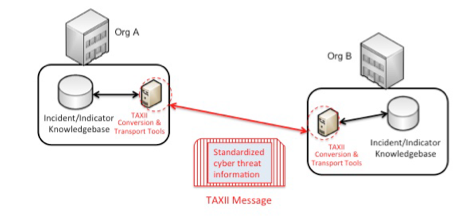
\includegraphics[width=150mm]{./Figures/TAXIIArchitecture1.png}
\end{figure}

 
 \subsection{Objetivos de TAXII}
 Los objetivos de TAXII son:
 \begin{itemize}
   \item Permitir el intercambio seguro y rápido de información referente a 
   amenazas entre comunidades de defensores de seguridad.
   \item Lograr un estándares para permitir compartir indicadores entre otros 
   elementos entre organizaciones.
   \item Extender el intercambio de indicadores para permitir intercambios 
   seguros, robustos y de gran volumen que tengan una expresividad mayor a la 
   actual.
   \item Soportar un amplio número de casos de uso y practicas comunes a las 
   comunidades.
   \item Tomar los estándares existentes que sean adecuados.
   \item Llegar a una adopción por parte de organizaciones internacionales de 
   estándares.
 \end{itemize}
 
 TAXII no ha creado una comunidad para compartir, sino que permite que las 
 comunidades compartan. TAXII mejora las deficiencias existentes proveyendo 
 especificaciones abiertas y comunes para transportar los mensajes con 
 información con capacidades como encriptación, autenticación, 
 direccionamiento, alertas y pedidos entre sistemas.
  
  \subsection{Representación estándar de la información}
TAXII utiliza el lenguaje STIX para representar la información. STIX es un 
lenguaje desarrollado por la comunidad para la especificación, captura, 
caracterización y comunicación de información de amenazas cibernéticas de forma 
estandarizada. STIX provee una arquitecutra unificada que soporta varios tipos 
de información entre los cuales se incluyen Cyber Observables, Indicadores, 
Incidentes, tácticas, técnicas y procedimientos de los adversarios, etc.

Para maximizar la compatibilidad y facilidad de adopción, STIX utiliza varios 
standards como CybOX, Common vulnerabilities and exposures (CVE) y common 
platform enumeration (CPE).

\subsection{Un framework de Intercambio}
La segunda parte necesaria para automatizar el intercambio de información es 
especificar como esta es compartida. Para alcanzar esto, TAXII define 
especificaciones técnicas y documentación de soporte. En particular, las 
especificaciones de TAXII definen un conjunto de capacidades necesarias para el 
transporte exitoso de mensajes, o como los mensajes TAXII llegan del punto A al 
B. Los mensajes TAXII llevan datos de amenazas informáticas transformadas a 
formato STIX. El conjunto completo de los mensajes incluye mensajes con datos y 
de control.

TAXII utiliza protocolos y especificaciones existentes siempre que sea posible y 
los integra con los mecanismos actuales para reducir los costos de 
implementación y permitir una adopción rápida por parte de las organizaciones ya 
establecidas que ya comparten información. TAXII esta siendo desarrollado de 
forma modular para soportar una variedad de mecanismos y formatos de datos para 
ser intercambiados.

\subsection{Casos de Uso}
TAXII ha sido desarrollado para soportar casos de uso comunes para el 
intercambio de información.

Alertas o Advertencias públicas

Estas son advertencias al publico en general o a varios asistentes de varios 
CSIRT, enviadas a todos los suscriptores.
Estas alertas son de una naturaleza tan amplia que no necesitas ser encriptadas 
o no se necesitan autorizaciones. Sin embargo es importante una firma digital  
para asegurar la autenticidad. Las entidades u organizaciones deben ser 
especificadas para identificar la fuente de la alerta.

Alertas y Reportes privados

Las alertas privadas son similares a las públicas, exceptuando que la 
información compartida es sensible y restringida a los socios que comparten 
datos. Los mecanismos para enviar datos deberían ser similares a los de las 
alertas públicas. Como las alertas y reportes se suponen sensibles y no para el 
uso general, es importante que TAXII soporte formas adecuadas de encriptación, 
autenticación, autorización e identificación de datos. Dependiendo en la 
naturaleza de las comunicaciones, manejo explícito de marcas o restricciones 
en datos compartidos debería ser necesario.

Las alertas son generalmente cortas, mensajes estándares con indicadores muy 
específicos o acciones especificadas.

Los reportes son mensajes mas largos, y pueden incluir reportes de incidentes, 
análisis de malware, análisis de amenazas u otras observaciones.

Soportes para Queries

Es común que los analistas de amenazas busquen información de otros entre sus comunidades
así como por fuera de ellas.
\begin{itemize}
  \item RFI (Request for Information): es un mensaje simple que se espera sea 
  manejado de forma manual y que permite que se pida información.
  \item Repository Search: Para este tipo de query, es esperado que una 
  organización ofrezca repositorios en los que buscar, los cuales podrían ser 
  compatibles con TAXII o STIX.
\end{itemize}

\subsubsection{Transferencia}

Varias organizaciones que transfieren información necesitan en algunas 
instancias agregar miembros. El nuevo miembro necesitas obtener los datos del 
repositorio de la organización. Por ello se desea un caso de uso para realizar 
el intercambio de un gran volúmen de datos.

\section{Componentes de TAXII}
\begin{itemize}
  \item Especificación de TAXII: Define la especificación de los componentes y 
  provee guía y requerimientos sobre como dichas especificaciones interoperan en 
  TAXII.
  \item Especificación de servicios de TAXII: Define una serie de servicios que 
  deben ser implementados para ser compatible con TAXII. Describe información 
  intercambiada a un nivel alto y no se limita a ningún mecanismo de 
  intercambio en especial.
  \item Implementación de Servicios: Se realiza una implementación de los 
  servicios TAXII para un mecanismo de intercambio. Cada implementación de 
  servicios provee guía técnica y requerimientos para implementar la 
  especificación de los mecanismos de intercambio.
  \item Modelo de datos de mensajes: Se define una estructura para los mensajes 
  TAXII, incluyendo header, payload, control y mensajes de datos. Los mensajes 
  de datos utilizan STIX para el payload de los mensajes TAXII.
  \item Implementaciones de los mensajes de datos: Es una implementación del 
  modelo de datos de mensajes, incluyendo el payload STIX.
   Cada implementación de mensajes define la guía técnica y 
  requerimientos  para utilizar un formato de mensajes particular para expresar 
  el modelo de datos de mensajes.
\end{itemize}

\subsection{TAXII Toolkit}
Es provisto para soportar la adopción de TAXII y asistir en el desarrollo de 
capacidades compatibles. El toolkit provee una colección de implementaciones de 
referencia, un conjunto de herramientas y una colección de librerías e 
interfaces.

\Section{Especificaciones de TAXII}

TAXII esta definido por múltiples especificaciones relacionadas. Esta sección 
describe las especificaciones definidas en TAXII.

\begin{itemize}
  
\item Especificación de Servicios (Service Specification): Provee los requerimientos por los cuales se definen los servicios e intercambios 
de TAXII. No provee detalles respecto al formato de los datos o como los 
mensajes TAXII son transportados por la red. Dichos detalles y requerimientos 
pueden ser encontrados en Protocol Binding Specification y Message Binding 
Specification.
\item Especificación de protocolos de enlace (Protocol Binding Specification): 
Define los requerimientos para transportar mensajes TAXII por la red. Puede 
haber varias especificaciones creadas para TAXII. Cada especificación define 
requerimientos para transportar mensajes TAXII usando protocolos de red y se 
proveen requerimientos respecto a como los servicios TAXII son soportados por 
los protocolos de red.
\item Especificación de Mensajes (Message Binding Specification): Se definen 
requerimientos para representar mensajes TAXII en un formato particular. Puede 
haber múltiples especificaciones para dichos mensajes. Se provee información 
detallada sobre como la información definida en la especificación de servicios 
es expresada en los mensajes.
\end{itemize}

\begin{figure}[ht!]
  \centering
    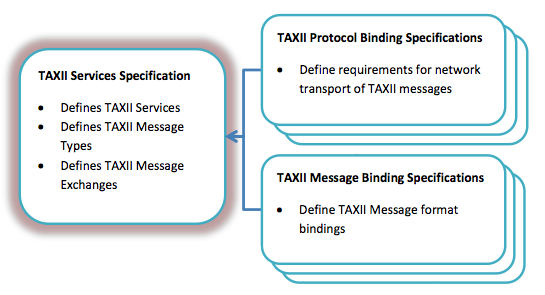
\includegraphics[width=150mm]{./Figures/TAXIIEspecification.png}
\end{figure}


Separación de la especificación de servicios, los protocolos de enlace y los 
mensajes existe para dar flexibilidad mientras TAXII evoluciona. Debido a que 
las organizaciones generalmente tienen restricciones respecto a los protocolos 
que soportan, TAXII busca no ligarse a un único protocolo que excluya a una 
parte de la comunidad. Cuando se ve que la comunidad expresa interés en un nuevo 
protocolo o tipo de mensaje, TAXII puede dar soporte para ellos sin cambiar los 
componentes centrales.

Dos grupos que usen el mismo protocolo de red y formato de mensajes serán 
capaces de intercambios de información estructurada de forma automática. Las 
políticas de intercambio de los participantes puede limitar estos intercambios 
si es necesario, pero el uso de servicios compatibles con TAXII asegura que 
se puede intercambiar cualquier información con los mecanismos definidos por 
TAXII. Los grupos que usen diferentes protocolos o formatos de mensajes no serán 
capaces de comunicarse directamente, pero como están utilizando mensajes y 
servicios en el núcleo de las comunicaciones de sus comunidades significa que es 
posible establecer caminos para que ocurra la interacción.

\subsection{Especificación de Servicios}
Esta especificación provee normativas respecto a los servicios, mensajes e 
intercambio de mensajes en TAXII. No provee detalles respecto a como los 
mensajes son transportados, dejando eso a la especificación de los protocolos de 
enlace. Si bien se provee información relacionada a la información presente en 
los mensajes TAXII, no da información respecto a como los mensajes TAXII son 
expresados.


\subsubsection{Unidades funcionales de TAXII}


Las unidades funcionales de TAXII representan conjuntos discretos de actividades 
requeridas para soportar TAXII. Una unidad funcional representa algún componente 
con un rol bien definido en TAXII.

\begin{itemize}
  \item TAXII Transfer Agent (TTA) : Es una unidad funcional conectada a la red 
  que envía o recibe mensajes TAXII. Una TTA interactúa con otras TTAs por medio 
  de la red y maneja los detalles de los requerimientos del protocolo de uno o 
  más TAXII Protocol Binding Specifications. Una TTA provee mensajes TAXII a un 
  TAXII Message Handler permitiendo que este último sea independiente del 
  protocolo de red utilizado. De la misma forma, el TTA puede ser independiente 
  del contenido de los mensajes TAXII, dejando el manejo de la información al 
  TAXII Message Handler.
  \item TAXII Message Handler (TMH): Es una unidad funcional que produce y 
  consume mensajes TAXII. El TMH es responsable de parsear y construir mensajes 
  con el formato especificado en uno o mas TAXII Message Binding Specifications. 
  Un TMH interactúa con un TTA, el cual maneja los detalles necesarios para 
  transmitir mensajes por la red. El Back-end TAXII interactúa con el TMH para 
  convertir su contenido en mensajes TAXII, y llevar a cabo actividades basadas 
  en los mensajes TAXII que son recibidos por el TMH.
  \item TAXII Back-end: Cubre todas las unidades funcionales distintas al TTA y 
  al TMH. Las especificaciones de TAXII no proveen requerimientos sobre como son 
  implementadas las capacidades en un back-end mas allá de como debe interactuar 
  con el TMH. Las organizaciones o implementadores pueden decidir que 
  capacidades implementar según los servicios TAXII que deseen soportar o según 
  como quieren dar ese soporte.
  \item Arquitectura TAXII: Cubre los aspectos de las unidades funcionales de la 
  infraestructura de productor o consumidor que prove o utiliza servicios TAXII. 
  Una arquitectura TAXII incluye una TTA, un TMH y un back-end TAXII.
  
  
\begin{figure}[ht!]
  \centering
    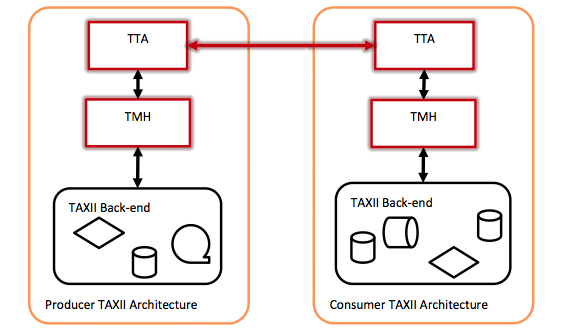
\includegraphics[width=150mm]{./Figures/TAXIIArchitecture.png}
\end{figure}
  
\end{itemize}

\subsubsection{Roles en TAXII}

Los roles en TAXII son utilizados de acuerdo al uso que se hace de los servicios 
especificados en TAXII.
\begin{itemize}
  \item Productor es el rol de una entidad que es la fuente de información 
  estructurada de amenazas.
  \item Consumidor es el rol de la entidad que recibe información estructurada 
  sobre amenazas.
\end{itemize}

\subsubsection{Componentes de red}

Los siguientes términos son utilizados para definir componentes de una 
implementación TAXII utilizando un modelo cliente-servidor.
\begin{itemize}
  \item Una implementación TAXII es un implementación específica de una 
  arquitectura TAXII.
  \item Servidor TAXII Es una implementación que provee uno o mas servicios 
  TAXII. Para soportar esta funcionalidad, se asume que un servidor TAXII esta 
  continuamente esperando tráfico de red.
  \item Cliente TAXII Es una implementación TAXII que inicia intercambio con un 
  servidor TAXII. Un cliente no necesita una conexión persistente con Internet 
  para operar pero puede abrir conexiones cuando desea interactuar con un 
  servidor y desconectarse de Internet cuando la conexión a terminado.
  \item TAXII endpoint denota una implementación TAXII que puede ser un servidor 
  o un cliente
\end{itemize}


\subsection{Capacidades}
La existencia de TAXII provee capacidades especificas para aquellos que desean 
compartir información de amenazas cibernéticas. Las capacidades TAXII son el 
nivel mas alto en el cual se pueden expresar las acciones de TAXII. Hay tres 
capacidades que soporta la actual versión de TAXII: push messaging, pull 
messaging y discovery.

\subsubsection{Push Messaging}

La información puede ser enviada de un productor a un consumidor. Esto puede 
reflejar una relación pre-existente entre el productor y el consumidor en la que 
el consumidor a pedido que se le envíen datos desde el productor. También puede 
usarse en caso de que el consumidor desee aceptar contribuciones de cualquier 
productor, y estos le envíen datos en cualquier momento.

\subsubsection{Pull Messaging}

Un consumidor puede requerir información de un productor. Esto no solo le 
permite al consumidor el control sobre el momento en el que recibe los datos 
sino que también le permite hacerlo sin tener que aceptar conexiones entrantes. 
Así como en push messaging, el productor y consumidos pueden tener acuerdos 
pre-existentes  para que el consumidor tenga acceso a los datos del productor. 
De forma alternativa, un productor puede hacer su información pública  y 
cualquer consumidor puede requerir sus datos.
La versión actual de pull messaging, limita a los consumidores a hacer pedidos 
por medio de las organizaciones productoras de los datos en lugar de por los 
datos en si. Todos los datos provistos por un productor deben estar organizados 
en grupos llamados "TAXII Data Feeds". Piezas individuales de información en un 
TAXII Data Feed son etiquetadas utilizando timestamps. El productor tiene total 
discresión sobre como el contenido se mapea en TAXII Data Feeds y en el 
significado de los timestamps. La capacidad de pull messaging esta atada a 
entender el contenido del productor.

\subsubsection{Discovery}

Para facilitar las comunicaciones automatizadas, TAXII soporta capacidades para 
descubrir los servicios específicos que ofrece un servidor o grupo de 
servidores, así como los protocolos o mensajes que este servidor ofrece. Esto no 
quita la necesidad del involucramiento humano para establecer acuerdos de 
cooperación lo cual esta por fuera del objetivo de TAXII. Sin embargo permite el 
intercambio de información respecto a las capacidades que un productor pudiera 
soportar y cuales son los mecanismos que utiliza para hacerlo.


\subsection{Servicios TAXII}
Los servicios TAXII representan un conjunto de mecanismos necesarios para 
soportar capacidades TAXII. Una implementación TAXII pudiera implementar alguno, 
todos o incluso ninguno de los servicios definidos.
TAXII define los siguientes servicios:
\begin{itemize}
  \item Servicio de descubrimiento: Es utilizado para recibir y responder a 
  mensajes que requieren información sobre los servicios ofrecidos.
  \item Feed Managment Service: Es utilizado para recibir o responder a mensajes 
  utilizados para el manejo de subscripciones a TAXII Data Feed.
  \item Inbox Service: Es utilizado para recibir información de amenazas 
  cibernéticas por medio de intercambios iniciados por el productor en intervalos 
  dictados por este.
  \item Poll Service: Es utilizado para recibir y responder a mensajes de pedido 
  a el TAXII Data Feed iniciados por el consumidor.
\end{itemize}

A continuación se describen los distintos servicios.

\subsubsection{Discovery Service}

Es un mecanismo para comunicar información referente al uso de servicios TAXII y 
a su disponibilidad. Para un pedido al servicio, se retorna una lista de los 
servicios TAXII y como estos pueden ser invocados. Un solo servicio de 
descubrimiento puede reportar servicios TAXII en diferentes equipos finales o 
incluso en múltiples organizaciones, los propietarios del servicio pueden 
definir su alcance a gusto. Un servicio de descubrimiento puede utilizar 
varios factores para determinar cuales servicios revelar ante una petición, 
incluyendo, pero no limitado a la entidad del cliente TAXII.
El servicio de descubrimiento debe soportar "Discovery Message Exchange".

\subsubsection{Feed Managment Service}

Es el mecanismo con el cual un consumidor pide información referente a TAXII 
Data Feeds, pidiendo subscripciones a estos, o modificando las existentes. Éste 
servicio facilita el intercambio de mensajes para manejar las subscripciones. 
No se entrega contenido de los TAXII Data Feed, en su lugar se envia 
contenido del TAXII Data Feed al servicio de Inbox de un consumidor en intercambios 
iniciados por un productor o en respuesta directa a un pedido del consumidor al 
servicio de poll.
Dicho servicio debe implementar soporte para subscription managment exchange.
Dicho servicio podría implementar soporte de feed information exchange.

\subsubsection{Inbox service}
Éste servicio es el mecanismo con el cual un consumidor acepta los mensajes en 
un intercambio iniciado por el productor. Un consumidor puede implementarlo 
para recibir datos del TAXII Data Feed.
El servicio de inbox debe implementar soporte para Data Push Exchange.

\subsubsection{Poll service}
Es provisto por un productor para permitir pedidos al TAXII Data Feed iniciados 
por  el consumidor. Un consumidor contacta a éste servicio explícitamente 
pidiendo el contenido del TAXII Data Feed. Los productores podrían ofrecer Data 
Feeds combinando envios al Inbox service del consumidor o por medio de pedidos 
al servicio de poll de productor.
Un implementación de éste servicio debe dar soporte a Data Poll Exchange.


\section{Intercambio mensajes TAXII}
Esta sección describe los mensajes de intercambio TAXII necesarios para soportar 
los servicios TAXII definidos antes. Estos intercambios solo consideran mensajes 
TAXII y son independientes a los protocolos sobre los cuales viajan los mensajes 
TAXII. En particular, esos protocolos podrían requerir intercambios de red 
adicionales antes de transmitir mensajes TAXII o romper un mensaje TAXII en 
multiples mensajes del protocolo subyacente que son transmitidos 
independientemente. Los siguientes diagramas representan conceptualmente la 
secuencia en la cual los mensajes TAXII son transmitidos y como actúan.

\subsection{Data Push Exchange}
En este intercambio, un mensaje STIX es transmitido desde un cliente a un 
servidor Inbox que este esperando. El mensaje STIX puede ser solicitado o no 
solicitado. El servidor inbox puede ser capaz de filtrar mensaje basandose en la 
autenticidad del emisor. Los mensajes enviados en este intercambio no deberian 
tener un campo 'In Response to' en su header.

\begin{figure}[ht!]
  \centering
    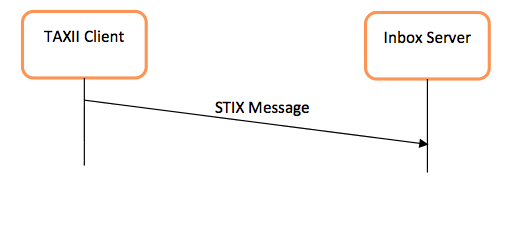
\includegraphics[width=150mm]{./Figures/DataPushExchange.png}
\end{figure}

El cliente TAXII envia un mensaje STIX al inbox server. El inbox server podria 
descartar el mensaje o pasar el mensaje STIX junto con cualquier información de 
la entidad autenticada al Back-end TAXII. El cliente TAXII no recibe respuesta 
del servidor de inbox y no sabra si el mensaje ha sido aceptado o descartado por 
el servidor, aunque el protocolo confiable de la capa inferior puede asegurar 
que el mensaje fue entregado a la TTA del servidor de inbox. El inbox server no 
enviara un mensaje de error TAXII si hay algún problema con el mensaje TAXII.

\subsection{Discovery Exchange}
Un cliente TAXII pide información sobre el servicio TAXII ofrecido por un 
productor. El discovery server del productor responde con una lista de 
servicios. Si bien el cliente puede ser informado de la existencia de un 
servicio, este no necesariamente tendrá acceso inmediato al servicio.

\begin{figure}[ht!]
  \centering
    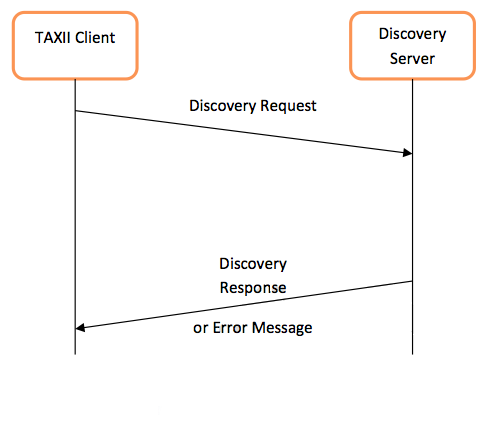
\includegraphics[width=150mm]{./Figures/DiscoveryExchange.png}
\end{figure}

El cliente TAXII envia un pedido de descubrimiento al servidor. Cuando el 
servidor recibe el pedido puede retornar un mensaje de error o pasar la 
información al Backend TAXII. Información relevante incluye la identidad 
autenticada si ésta fue provista. El Backend TAXII podría utilizar esta 
información junto a su propia política de control de acceso  para crear una 
lista de servicios a ser retornada. Esto podría ser empaquetado en una 
respuesta de discovery lo cuales podrían ser enviados al cliente TAXII. El 
cliente TAXII recibe esa respuesta y la pasa la información del servicio a su 
propio Back-End para ser procesado.

\subsection{Feed Information Exchange}

En este intercambio un cliente TAXII pide información sobre fuentes de datos disponibles en 
un Feed Server. El servidor responde con una lista de fuentes de datos 
disponibles. Dicha respuesta es realizada por back-end y se pueden considerar 
decisiones de control de acceso para realizar la respuesta.

\begin{figure}[ht!]
  \centering
    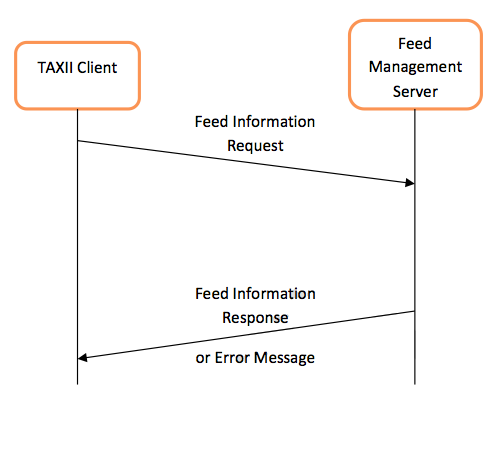
\includegraphics[width=150mm]{./Figures/FeedInformationExchange.png}
\end{figure}

En este intercambio, el cliente TAXII envia el Feed Information Request al 
servidor. Cuando el servidor recibe la request podría retornar un mensaje de 
error o pasar la información relevante al TAXII Back-end. Entre la información 
relevante se podría incluir la identidad. El Back-end podria utilizar esta 
información junto con sus políticas de control de acceso para crear una lista de 
fuentes de datos para ser enviadas al cliente. Esta lista es empaquetada en una 
Feed Information Response. El cliente recibe este mensaje y pasa el Feed a su 
propio Back-end para ser procesado.

\subsection{Subscription Managment Exchange}

En este un cliente intenta establecer, borrar, pausar, resumir o modificar una 
subscripción a un TAXII Data Feed conocido enviando un mensaje subscription 
managment request al servidor. El servidor pasa la request al TAXII Back-end el 
cual determina la respuesta. Esta respuesta es luego enviada al cliente.

\begin{figure}[ht!]
  \centering
    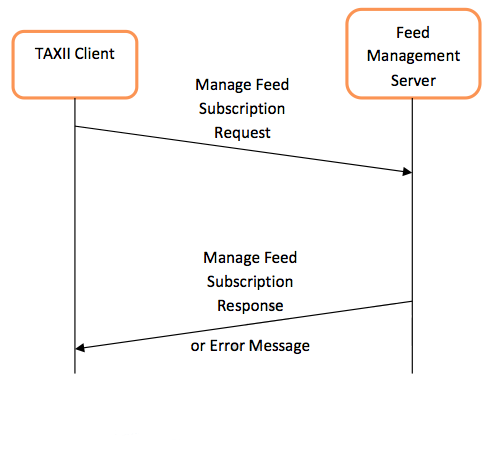
\includegraphics[width=150mm]{./Figures/SubscriptionManagmentExchange.png}
\end{figure}

El cliente TAXII envia una Manage Feed Subscription Request al servidor. Este 
podría retornar un mensaje de error TAXII o pasar la información relevante al 
TAXII Back-end. La información relevante podría incluir la identidad, parámetros 
que identifiquen la subscripción a ser modificada o creada, y la acción 
realizada. El Back-end TAXII puede usar dicha información junto con sus 
políticas de control de acceso y las funcionalidades que posea para determinar 
si la acción esta permitida o no. Dependiendo en la respuesta, el servidor 
podría retornar un mensaje de error TAXII o enviar una respuesta Manage Feed 
Successful Response.

\subsection{Feed Poll Exchange}

Es utilizado por un consumidor para pedir contenido de un productor de datos. El 
TAXII Data Feed content es enviado al consumidor en el mismo intercambio. Esto  
permite a un consumidor devolver el Data Feed Content en su propia tabla de 
tiempo y sin necesidad de utilizar un Inbox Server o aceptar conexiones 
entrantes.

\begin{figure}[ht!]
  \centering
    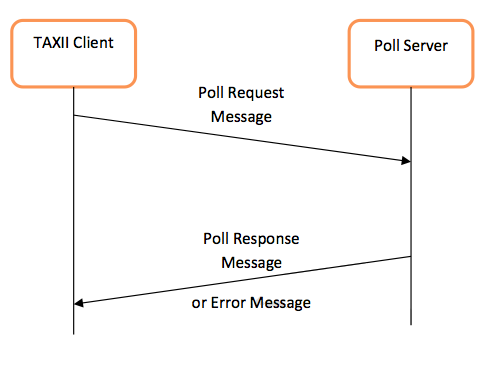
\includegraphics[width=150mm]{./Figures/FeedPollExchange.png}
\end{figure}

El cliente consumidor inicia el intercambio enviando un mensaje Poll Request al 
servidor de Poll del productor. El servidor puede enviar un mensaje de error 
inmediatamente o pasar la información relevante al TAXII Back-end. Información 
relevante incluye el nombre de la fuente, los parámetros de subscripción, 
timestamps indicando el intervalo de tiempo de la información que pide el 
consumidor y la identidad del consumidor. El back-end TAXII evalua esta 
información para determinar la respuesta. Hay tipos de respuesta posibles:
\begin{itemize}
  \item El pedido de información podria ser denegado. En este caso el servidor 
  de poll crea un error TAXII 
  \item Un conjunto de contenido TAXII Data Feed podria ser provisto. En este 
  caso , el servidor de Poll construira y enviara un mensaje de Poll Response. 
  Este mensaje indica el intervalo de tiempo que cubre el TAXII Data Feed que es 
  transmitido y los cuerpos de mensajes STIX que forman el contenido del TAXII 
  Data Feed.
\end{itemize}
En todos los casos, el cliente TAXII recibe el mensaje apropiado y pasa esta 
información al Back-end TAXII para ser procesado.

\section{Uso de TAXII}

Anteriormente se identifican distintos modelos utilizados por las comunidades para el 
el intercambio de información de amenazas informáticas. Estos modelos son 
Source/Suscriber, Peer-to-peer y Hub and Spoke. A continuación se  muestre como 
los servicios TAXII pueden ser utilizados para la implementación de dichos 
modelos.

\subsection{Source/Suscriber}

En este modelo una entidad es la fuente de información y algunos subscriptores 
tienen acuerdos con dicha entidad para recibir información periódicamente. Es 
deseado que los subscriptores no se conozcan entre si, para ello la fuente 
realiza acuerdos con cada uno de los subscriptores. En este modelo, la fuente es 
un productor TAXII mientras que los subscriptores son consumidores.

TAXII soporta este tipo modelo de intercambio con el uso de los servicios de 
Discovery, Feed Management, Inbox y Poll. Una organización que desee 
subscribirse al TAXII Data Feed de la fuente necesita conocer los servicios 
TAXII que la fuente ofrece y como contactar con ellos. Si bien esto podría ser 
realizado por una mecanismo fuera de banda (Publicar la información en otro medio)
también podría ser logrado contactando al servicio Discovery de la fuente. Desde 
este punto, el subscriptor podría contactar al servicio de Feed Managment 
identificado para aprender que fuentes ofrece el productor y que restricciones 
podría tener su acceso.

Si el contenido del TAXII Data Feed es restringido solo a algunas entidades 
autorizadas y el productor ha determinado que el subscriptor tiene permitido 
recibir el contenido, la fuente y el subscriptor necesitan acordar en como el 
subscriptor se autenticara. Dependiendo en el protocolo que soporta la fuente, 
esto se puede realizar por medio de una contraseña, un certificado o por otros 
medios. Si el contenido de un TAXII Data Feed es abierto y no requiere 
autenticación, este paso es innecesario cuando se establecen las subscripciones 
al TAXII Data Feed.

Una vez que la fuente es es capaz de autenticar al subscriptor (si es 
necesario), el subscriptor puede contactar al Feed Managment Service del 
productor y pedir subscripciones a las fuentes del productor. La fuente puede 
comparar dichos pedidos con su propio entendimiento de lo que el subscriptor 
puede recibir y permitir o denegar dichos pedidos según corresponda. La fuente 
puede enviar contenido al subscriptor al Inbox Service de este en el intervalo 
apropiado. Alternativamente, el subscriptor podría contactar al Poll service de 
la fuente para descargar el contenido deseado.

\begin{figure}[ht!]
  \centering
    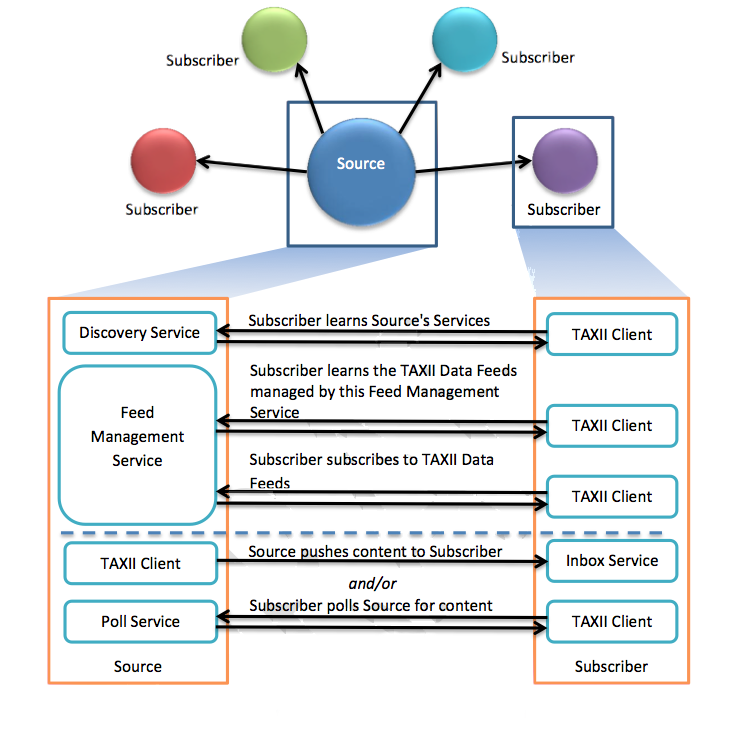
\includegraphics[width=150mm]{./Figures/SourceSuscriberModel.png}
\end{figure}

La figura mostrada como el modelo Source/Subscriber puede ser soportado por los 
servicios TAXII. El diagrama muestre los mensajes TAXII intercambiados entre la
fuente y el subscriptor. Con los intercambios que están por encima de la línea 
punteada se establece la subscripción. Los intercambios pueden ser realizados 
repetidamente sin la necesidad de realizar el proceso de subscripción 
nuevamente.

\subsection{Peer-to-peer}

En un modelo Peer-to-peer, los pares de organizaciones entran en un acuerdo 
mutuo para compartir su información entre ellos. En este modelo, cada Peer puede 
operar como productor y consumidor. Los socios en este intercambio podrían 
establecer fuentes utilizando un procedimiento similar al establecido en el 
modelo Source/Subscriber. Alternativamente, podrían acordar subir o descargar 
contenido sin ninguna subscripción formal. No tener una subscripción formal 
permitiria a un Peer albergar un Inbox Service sin necesidad de un Feed 
Managment Service.

El modelo Peer-to-Peer tiene dos variantes: acuerdos para el intercambio entre 
comunidades y acuerdos para el intercambio ad-hoc. En el primero la comunidad 
constituye acuerdos entre pares en los que todos los miembros acuerdan una única 
política la cual seguirán todos los miembros. A diferencia de los otros dos 
modelos que tienen un punto central desde el cual la información es diseminada, 
todo el intercambio ocurre de forma punto a punto entre los pares. Si dos pares 
cualquiera desean recibir información de otro directamente, estos necesitaran 
establecer un acuerdo apropiado con el otro para que el Peer le envíe 
información.

Alternativamente, el intercambio entre pares puede ser realizado de forma 
individual con intercambios ad-hoc. Esto podría ocurrir si dos compañías hacen 
acuerdos individuales para compartir entre ellas. En este caso, los acuerdos 
sobre que compartir son específicos para las partes. Una sola entidad podría 
participar en ambas variantes, perteneciendo a una o mas comunidades en las 
cuales los miembros comparten entre si siguiendo un acuerdo común entre los 
miembros y a su vez negocian acuerdos individuales con otras entidades. Alguna 
información recibida por medio de un acuerdo no siempre debería ser compartida 
con otros peers que no son parte del acuerdo. De esta forma un participante 
debería hacer un seguimiento de quien fue el proveedor de la información 
recibida, como se realiza ese seguimiento esta por fuera de la especificación de 
TAXII.

\begin{figure}[ht!]
  \centering
    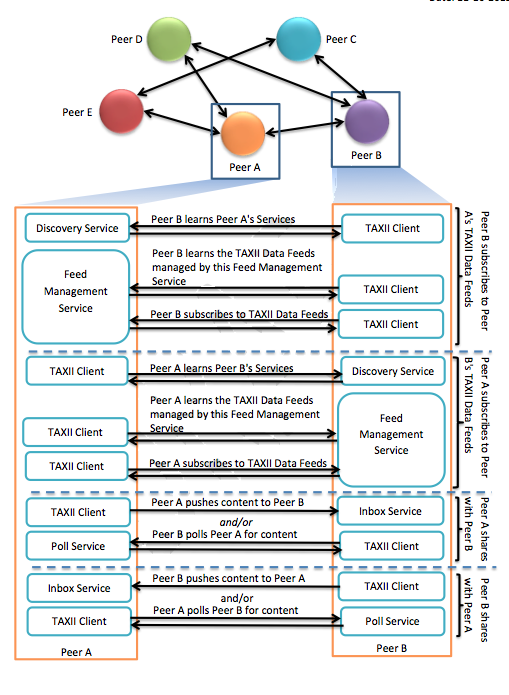
\includegraphics[width=150mm]{./Figures/PeerToPeerModel.png}
\end{figure}
\newpage
La figura anterior muestra como puede ser realizado el modelo Peer to peer por 
medio de los servicios TAXII. En este diagrama se ve que dos peers se contactan 
para pedir subscripciones para obtener información. Se asume que ambos peers 
tienen un Feed Managment Service que es utilizado para manejar todos los 
pedidos de subscripción.

\subsection{Hub and Spoke}

En un modelo Hub and Spoke, en este modelo la entidad Hub es un consumidor dede 
información que le proveen así como un productor que brinda información a un 
Spoke. Una entidad Spoke podría ser un productor, dando información al Hub, un 
consumidor que reciba actualizaciones del Hub o ambas. El Hub puede utilizar un 
Inbox Service para recibir información de cualquiera que desee enviar 
información de forma voluntaria y/o podría requerir información de ciertas 
fuentes para guardar la información en una única ubicación. Desde este punto, el 
Hub puede funcionar como una entidad Source del modelo Source/Subscriber 
mientras que los Spoke serían Subscribers de dicho modelo. El Hub puede adoptar 
cualquier política respecto de la información que recibe, desde pasar toda la 
información automáticamente a solo pasar información de socios reconocidos, o 
realizar ediciones y análisis antes de re enviar la información.

\begin{figure}[ht!]
  \centering
    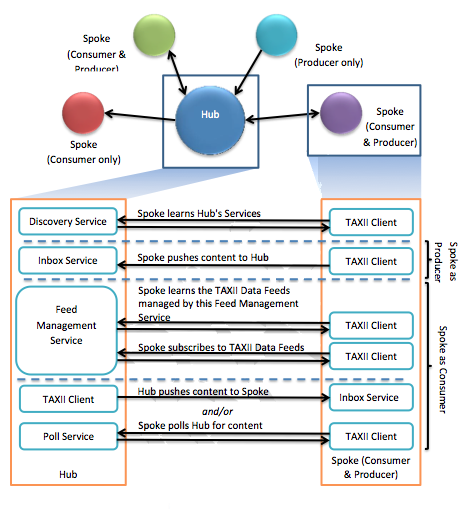
\includegraphics[width=150mm]{./Figures/HubAndSpokeModel.png}
\end{figure}
\newpage
La figura presentada muestra como se puede implementar el modelo Hub and Spoke 
utilizando los servicios provistos por TAXII. En este modelo algunas entidades 
Spoke podrían ser consumidores, otras productores y en algunos casos ambas. El 
diagrama muestra los intercambios que podrían ser utilizados por el Spoke que 
actúa como productor y consumidor. Si este desea actuar de una sola forma solo 
los intercambios necesarios serían relevantes. Independientemente del rol que 
tome el Spoke, es necesario que este conozca los servicios relevantes en el Hub. 
Esto se realiza utilizando el Discovery Service provisto por el Hub, de todas 
formas esto podría realizarse con mecanismos fuera de banda.

 
%% Chapter 1

\chapter{Glosario} % Main chapter title

\lfoot{Glosario}} % This is for the header on each page - perhaps a shortened title

%----------------------------------------------------------------------------------------



\emph{Conceptos utilizados en TAXII}
\begin{itemize}
  \item Botnet: Es una colección de computadoras comprometidas (llamadas computadoras zombie), 
instaladas generalmente mediante gusanos, troyanos y backdoors, controladas 
remotamente, usualmente con fines maliciosos, en especial para denegaciones de 
servicio.
  \item CSIRT: Es una organización responsable de recibir reportes de incidentes de seguridad, analizarlos y responder a ellos. [CERT/CC]
  \item CVE: El CVE (Common Vulnerabilities and Exposures) es un diccionario de comunes (por 
ejemplo los identificadores CVE) para publicar información conocida de 
vulnerabilidades de seguridad. El CCE (Common Configuration Enumeration) provee 
identificadores para problemas de configuración de seguridad. Los 
identificadores hacen más fácil compartir información a través de diferentes 
bases de datos y herramientas de seguridad.
 \item Cyber Threat information: Es cualquier información representable en STIX. 
 Esto incluye, pero no esta limitado a, Observables, Indicadores, incidentes, 
 TTPs (Tactics, Techniques y Procedures), exploit targets, campaigns, threat 
 actors y courses of action.
 \item TAXII Data Feed: Es una colección de cyber threat information 
 estructurada expresable en uno o mas documentos STIX que pueden ser 
 intercambiados utilizando TAXII. Cada TAXII Data Feed \emph{debe} tener un 
 nombre que lo identifica de forma única entre el resto de los feeds de un 
 productor dado. Cada elemento de un TAXII data feed debe ser etiquetado con un 
 timestamp y puede tener otras etiquetas a discreción del productor.
 \item IDS: Intrusion Detection System. Sistema que detecta intrusiones no deseadas en una 
red o equipo, que no pueden ser detectadas por un firewall convencional.
 \item Mensae TAXII: Un bloque de información que es pasado de una entidad a la 
 otra. Un mensaje TAXII representa un pedido o una respuesta.
 \item Intercambio de mensajes TAXII: Una secuencia definida de mensajes TAXII 
 intercambiados entre dos entidades.
\item Servicio TAXII: Son funcionalidades albergadas por algunas entidades y que 
es accedido o invocado usando uno o mas TAXII Message Exchange.
\item TAXII Capability: Una actividad de alto nivel soportado por TAXII por 
medio del uso de uno o mas servicios TAXII.
\end{itemize}




 
%\chapter{RTIR} % Main chapter title

\label{Chapter1} % For referencing the chapter elsewhere, use \ref{Chapter1} 

\lhead{\til}
\rhead{\fu}


%----------------------------------------------------------------------------------------

\section{Que es RTIR}
RTIR es un sistema de manejo de incidentes diseñado para ser utilizado por los 
equipos de seguridad de sistemas. A sido creado en conjunto con equipos de CERT 
y CSIRT para manejar el creciente número de incidentes reportados.
Presenta la ventaja de ser opensource, contener una API completa y una comunidad 
de usuarios grande y experta. Además es simple de integrar con otras 
herramientas existentes. Está implementado por medio de módulos PERL y las 
herramientas que provee RT. Se puede pensar en RTIR como una extensión de RT 
para ser utilizada por CERT's y CSIRT's.

Existen algunas alternativas a RTIR como lo son AIRT (Application for Incident Response Teams) 
cuya última versión data de Julio de 2009. AIRT es una aplicación web 
desarrollada para los equipos de respuesta a incidentes. Busca proveer facilidad 
ante los reportes de incidentes de seguridad así como un seguimiento simple de 
estos. Este sistema no cuenta con una comunidad comparable a la de RTIR así como 
con documentación tan extensa como la de RTIR.

Otra de las opciones existentes es OTRS (Open Technology Real Services), así 
como los anteriores también es open soruce. Presenta las ventajas de tener una 
comunidad más numerosa que AIRT y que el código esta siendo desarrollado continuamente. 
Así como RTIR esta desarrollado por medio de Perl y permite conectarse a varias 
bases de datos. Presenta documentación extensa para implementadores. 
%\input{./Chapters/Chapter7} 

%----------------------------------------------------------------------------------------
%	THESIS CONTENT - APPENDICES
%----------------------------------------------------------------------------------------

\addtocontents{toc}{\vspace{2em}} % Add a gap in the Contents, for aesthetics

\appendix % Cue to tell LaTeX that the following 'chapters' are Appendices

% Include the appendices of the thesis as separate files from the Appendices folder
% Uncomment the lines as you write the Appendices

%% Appendix A

\chapter{Appendix Title Here} % Main appendix title

\label{AppendixA} % For referencing this appendix elsewhere, use \ref{AppendixA}

\lhead{Appendix A. \emph{Appendix Title Here}} % This is for the header on each page - perhaps a shortened title

Write your Appendix content here.
%\input{./Appendices/AppendixB}
%\input{./Appendices/AppendixC}

%\addtocontents{toc}{\vspace{2em}} % Add a gap in the Contents, for aesthetics

\backmatter

%----------------------------------------------------------------------------------------
%	BIBLIOGRAPHY
%----------------------------------------------------------------------------------------

%\label{aaaa}

%\lhead{\emph{Bibliografia}} % Change the page header to say "Bibliography"
\nocite{*}
\bibliographystyle{plain} % Use the "unsrtnat" BibTeX style for formatting the Bibliography
\bibliography{bibliography} % The references (bibliography) information are stored in the file named "Bibliography.bib"

\end{document}  